% mnras_template.tex
%
% LaTeX template for creating an MNRAS paper
%
% v3.0 released 14 May 2015
% (version numbers match those of mnras.cls)
%
% Copyright (C) Royal Astronomical Society 2015
% Authors:
% Keith T. Smith (Royal Astronomical Society)

% Change log
%
% v3.0 May 2015
%    Renamed to match the new package name
%    Version number matches mnras.cls
%    A few minor tweaks to wording
% v1.0 September 2013
%    Beta testing only - never publicly released
%    First version: a simple (ish) template for creating an MNRAS paper

%%%%%%%%%%%%%%%%%%%%%%%%%%%%%%%%%%%%%%%%%%%%%%%%%%
% Basic setup. Most papers should leave these options alone.
\documentclass[a4paper,fleqn,usenatbib]{mnras}

% MNRAS is set in Times font. If you don't have this installed (most LaTeX
% installations will be fine) or prefer the old Computer Modern fonts, comment
% out the following line
\usepackage{newtxtext,newtxmath}
% Depending on your LaTeX fonts installation, you might get better results with one of these:
%\usepackage{mathptmx}
%\usepackage{txfonts}

% Use vector fonts, so it zooms properly in on-screen viewing software
% Don't change these lines unless you know what you are doing
\usepackage[T1]{fontenc}
\usepackage{ae,aecompl}


%%%%% AUTHORS - PLACE YOUR OWN PACKAGES HERE %%%%%

% Only include extra packages if you really need them. Common packages are:
\usepackage{graphicx}	% Including figure files
\usepackage{amsmath}	% Advanced maths commands
\usepackage{amssymb}	% Extra maths symbols

\usepackage{multirow}
\usepackage{todonotes}

%%%%%%%%%%%%%%%%%%%%%%%%%%%%%%%%%%%%%%%%%%%%%%%%%%

%%%%% AUTHORS - PLACE YOUR OWN COMMANDS HERE %%%%%

% Please keep new commands to a minimum, and use \newcommand not \def to avoid
% overwriting existing commands. Example:
%\newcommand{\pcm}{\,cm$^{-2}$}	% per cm-squared

%%%%%%%%%%%%%%%%%%%%%%%%%%%%%%%%%%%%%%%%%%%%%%%%%%

%%%%%%%%%%%%%%%%%%% TITLE PAGE %%%%%%%%%%%%%%%%%%%

% Title of the paper, and the short title which is used in the headers.
% Keep the title short and informative.
\title[Short title, max. 45 characters]{Evaluation of data compression techniques for the inference of
  stellar atmospheric parameters from high resolution spectra}

% The list of authors, and the short list which is used in the headers.
% If you need two or more lines of authors, add an extra line using \newauthor
\author[K. T. Smith et al.]{
Keith T. Smith,$^{1}$\thanks{E-mail: mn@ras.org.uk (KTS)}
A. N. Other,$^{2}$
Third Author$^{2,3}$
and Fourth Author$^{3}$
\\
% List of institutions
$^{1}$Royal Astronomical Society, Burlington House, Piccadilly, London W1J 0BQ, UK\\
$^{2}$Department, Institution, Street Address, City Postal Code, Country\\
$^{3}$Another Department, Different Institution, Street Address, City Postal Code, Country
}

% These dates will be filled out by the publisher
\date{Accepted XXX. Received YYY; in original form ZZZ}

% Enter the current year, for the copyright statements etc.
\pubyear{2015}

% Don't change these lines
\begin{document}
\label{firstpage}
\pagerange{\pageref{firstpage}--\pageref{lastpage}}
\maketitle

% Abstract of the paper
\begin{abstract}
We evaluate the utility of several data compression techniques
  for alleviating the curse-of-dimensionality problem in regression
  tasks where the objective is to estimate stellar atmospheric
  parameters from high resolution spectra in the 4000-8000 K range. We
  conclude that ICA and kernel-PCA perform better than the rest of the
  techniques evaluated for all compression ratios. We also assess the
  necessity to adapt the signal-to-noise ratio (SNR) of the training
  set examples to the SNR of each test spectrum and conclude that
  within the conditions of our experiments, only two such models are
  needed (SNR=50 and 10) to cover the entire range.
\end{abstract}

% Select between one and six entries from the list of approved keywords.
% Don't make up new ones.
\begin{keywords}
Dimensionality Reduction -- keyword2 -- keyword3
\end{keywords}

%%%%%%%%%%%%%%%%%%%%%%%%%%%%%%%%%%%%%%%%%%%%%%%%%%

%%%%%%%%%%%%%%%%% BODY OF PAPER %%%%%%%%%%%%%%%%%%

\section{Introduction}

The rapid evolution of astronomical instrumentation and the
implementation of extensive surveys have permitted the acquisition of
vast amounts of spectral data.  {The reduction and management of
  large spectral databases collected by large-area or all-sky surveys
  like Gaia/Gaia-ESO \citep{2006MNRAS.367..290J,2012Msngr.147...25G},
  RAVE \citep{2006AJ....132.1645S}, or APOGEE
  \citep{2011AJ....142...72E} require the use of automatic
  techniques for the consistent, homogeneous, and efficient
  extraction of physical properties from spectra. The availability
  of these huge databases opens new possibilities to better understand
  the stellar, Galactic, and extra-galactic astrophysics. Of
  special importance is the determination of intrinsic stellar
  physical properties, such as effective temperature ($T_{\rm eff}$),
  surface gravity (log \textit{g}) and metallicity ([M/H]). However,
  the difficulty that atmospheric parameter estimation poses comes
  from the inherent size and dimensionality of the data. 
  Regression from stellar spectra suffers the so-called {\sl curse
  of dimensionality} problem because the number of variables
  (wavelengths) is much higher than the number of training samples.
    
The \textit{curse of dimensionality} \citep{bellman:61} relates to 
the problem caused by the exponential increase in volume associated 
with adding extra dimensions to Euclidean space. 
When the dimensionality increases, the volume of the space increases so 
fast that the available data become sparse. Because this sparsity is 
problematic for any method that requires statistical significance, the 
amount of data needed to support the result often grows exponentially 
with the dimensionality in order to obtain a statistically sound and 
reliable outcome.

Furthermore, typical spectra obtained in many surveys do not 
regularly reach the high signal-to-noise ratios (SNR) --about
100 or greater -- needed to obtain robust estimates, which
increases the difficulty to accurately estimate the physical
parameters of spectra.  In summary, stellar spectra are high
dimensional noisy vectors of real numbers and thus,
regression models must be both computationally efficient and robust
to noise.


There are several ways to alleviate this so-called curse of dimensionality. It is evident that not all wavelength bins in an observed spectrum carry the same amount of information about the astrophysical parameters of the stellar atmosphere. Astronomers have historically used features of the spectrum such as flux ratios (be them in the wavelength regions of individual spectral lines or absorption bands) to infer temperatures, gravities or metallicities (citation needed). That way, they reduce the full vector of fluxes to one value that is used to infer the astrophysical parameter of interest via a previously assumed 
calibration. Of course, there is no reason why one should restrict to one single value, and recent works based on machine learning techniques use several such spectral features to infer the astrophysical parameters (see e.g. \citep{2006ApJ...636..804A}).


The most popular dimensionality reduction technique applied
to stellar spectra is Principal Component Analysis (PCA). It has
been widely applied in spectral classification combined with
artificial neural networks (ANNs) \citep{singh:98} or support vector
machines (SVM) \citep{fiorentin:08b}. For continuum emission, PCA has a
proven record in representing the variation in the spectral properties
of galaxies. However, it does not perform well when reconstructing
high-frequency structure within a spectrum \citep{vanderplas:09}. To
overcome this difficulty, other methods have been used in the
spectral feature extraction procedure. Locally linear embedding
(LLE) \citep{roweisLLE:00} and Isometric feature map (Isomap) 
\citep{tenenbaum:00} are two widely used nonlinear dimensionality 
reduction techniques. Some studies found that LLE is efficient in 
classifying galaxy spectra \citep{vanderplas:09} and stellar spectra 
\citep{daniel:11}. Other authors concluded that Isomap performs better 
than PCA, except on spectra with low SNR (between 5 and 10) \citep{bu:14}.

A detailed study of data compression techniques has to include
the analysis of their stability properties against noise. In order
to improve the overall generalisation performance of the atmospheric
parameters estimators, experience shows that it is advantageous to
match the noise properties of the synthetic training sample to that of
the real sample because it acts as a regulariser in the training phase
\citep{fiorentin:08a}.  The impact of the SNR on the parameter
estimation ($T_{\rm eff}$, log \textit{g} and [Fe/H]) with artificial
neural networks (ANNs) is explored in \cite{snider:01}. They found
that reasonably accurate estimates can be obtained when networks are
trained with spectra --not derived parameters-- with similar SNR 
as those of the unlabelled data, for ratios as low as 13.

%Other approaches use a set of stellar spectra with a wide range of
%SNR by adding different levels of noise to each spectrum of the
%original catalog.

\cite{recio:06} determined three atmospheric parameters
($T_{\rm eff}$, log \textit{g} and [M/H]) and individual chemical
abundances from stellar spectra using the MATISSE (MATrix
Inversion for Spectral SynthEsis) algorithm. They introduced Gaussian
white noise to yield five values of SNR between 25 and 200 and found
that errors increased considerably for SNR lower than $\sim$ 25.  In
\cite{navarro:12} authors present a system based on ANNs trained with
a set of line-strength indexes selected among the spectral lines more
sensitive to temperature and the best luminosity tracers. They
generated spectra with a range of SNR between 6 and 200 by adding
Poissonian noise to each spectrum. Their scheme allows to classify
spectra of SNR as low as 20 with an accuracy better than two spectral
subtypes. For SNR $\sim$ 10, classification is still possible but at a
lower precision.

This paper presents a comparative study of the most popular
dimensionality reduction technique applied to stellar spectra (PCA)
and five alternatives (two linear and three nonlinear
techniques). The aims of the paper are (1) to investigate to what
extent novel dimensionality reduction techniques outperform the
traditional PCA on stellar spectra datasets, (2) to test the
robustness of these techniques and their performance in atmospheric
parameters estimation for different SNRs, (3) to investigate the
number of regression models of different SNRs needed to obtain the
best generalisation performance for any reasonable SNR of the test
data, and (4) to analyse the effect of the grid density over the 
performance in atmospheric parameters estimation.  
The investigation is performed by an empirical evaluation of
the selected techniques on specifically designed synthetic
datasets. In \ref{sec:dimred} we review the data compression
techniques evaluated in this work and their properties. In
Sect. \ref{sec:experiment} we describe the numerical experiments
carried out to evaluate these techniques, and in
Sect. \ref{sec:results} we present the main results from the
experiments. Finally, in \ref{sec:conclusions} we summarize the most
relevant findings from the experiments and discuss their validity
and limitations.

\section{Dimensionality reduction}
\label{sec:dimred}

For the sake of computational efficiency, and thinking in a 
dynamic environment, where a complete rerun of a dimensionality 
reduction algorithm becomes prohibitively time consuming, 
the selection of the dimensionality reduction techniques tested
  in our experiments was done amongst those capable of projecting new
  data onto the reduced dimensional space defined by the training set
  without having to re-apply the algorithm (process also known as 
  out-of-sample extension). Thus, in this work, we investigated three
linear dimensionality reduction techniques such as PCA, independent
component analysis (ICA) and discriminative locality alignment (DLA),
as well as three nonlinear reduction techniques that do not lack 
generalisation to new data: wavelets, Kernel PCA and diffusion maps (DM). 
We aimed at minimizing the regression
  error in estimating stellar atmospheric parameters with no
  consideration of the physicality of the compression
  coefficients. Physicality of the coefficients is sometimes
  required, for example, when trying to interpret galactic spectra as
  a combination of non-negative components.


Other linear and nonlinear techniques could be used for dimensionality 
reduction, such as linear discriminant analysis (LDA), locally linear 
embedding (LLE), Isomap, etc. When the number of variables is much 
higher than that of training samples, classical LDA cannot be directly 
applied because all scatter matrices are singular and this method 
requires the non-singularity of the scatter matrices involved. 
Isomap's performance exceeds the performance of LLE, specially when 
the data is sparse. However, in presence of noise or when the data 
is sparsely sampled, short-circuit edges pose a threat to both Isomaps 
and LLE algorithms \citep{saxena:04}. Short-circuit edges can lead to 
low-dimensional embeddings that do not preserve a manifold's true topology \citep{balasubramanianISOMAP:02}.

%Furthermore, Isomap and LLE lack a good 
%generalization property on new data points since they are defined only on 
%training data.

%\begin{itemize}
%\item PCA. Linear, unsupervised
%\item ICA. Linear, unsupervised
%\item DLA. Linear, supervised
%\item Diffusion Maps. Non-linear, preserving global properties
%\item Wavelets. Non-linear, preserving global properties
%\item Kernel PCA. Non-linear, preserving global properties
%\end{itemize}

\subsection{Principal Component Analysis (PCA)}

Principal Components Analysis (PCA) \citep{hotelling:33,pearson:01} is
by far the most popular (unsupervised) linear technique for
dimensionality reduction. The aim of the method is to reduce the
dimensionality of multivariate data whilst preserving as much of the
relevant information as possible. This is done by finding a linear
basis of reduced dimensionality for the data, in which the amount of
variance in the data is maximal.

PCA transforms the original set of variables into a new set of
uncorrelated variables, the principal components, which are linear
combinations of the original variables. The new uncorrelated variables
are sorted in decreasing order of variance explained. The first
new variable shows the maximum amount of variance; the second
new variable contains the maximum amount of variation unexplained by
the first one, and is orthogonal to it, and so on.  This is
achieved by computing the covariance matrix for the full data
set. Next, the eigenvectors and eigenvalues of the covariance matrix
are computed, and sorted according to decreasing eigenvalue.

\subsection{Independent Component Analysis (ICA)}

Independent Component Analysis (ICA) \citep{comon:94} is very closely
related to the method called blind source separation (BSS) or blind
signal separation \citep{jutten:91}. It is the identification and
separation of mixtures of sources with little prior information. The
goal of the method is to find a linear representation of non-Gaussian
data so that the components are statistically independent, or as
independent as possible \citep{hyvarinen:00}.

Several algorithms have been developed for performing ICA
\citep{bell:95,belouchrani:97,ollila:06,li:08}. A large widely used is
the FastICA algorithm \citep{hyvarinen:00} which has a number of
desirable properties, including fast convergence, global convergence
for kurtosis-based contrasts, and the lack of any step size parameter.
RobustICA algorithm \citep{zarzoso:10} represents a simple modification
of FastICA. This algorithm is based on the normalised kurtosis
contrast function, which is optimised by a computationally efficient
iterative technique. It is more robust than FastICA and has a very
high convergence speed.  Another widely used ICA algorithm is the
Joint Approximation Diagonalisation of Eigen matrices (JADE) algorithm
\citep{cardoso:93}. This approach exploits the fourth-order moments in
order to separate the source signals from mixed signals. This work
uses JADE algorithm for projecting the original spectra in the space
of independent components.


\subsection{Discriminative Locality Alignment (DLA)}
Discriminative Locality Alignment (DLA) \citep{zhang:2008} is a
supervised manifold learning algorithm, which can be divided into
three stages: part optimisation, sample weighting and whole
alignment. In the first stage, for each sample, one patch is built by
the given sample and its neighbours. On each patch DLA preserves the
local discriminative information through integrating two criteria:
that the distances between the intra-class samples will be as small as
possible and the distance between the inter-class samples will be as
large as possible. In the second stage, each part optimisation is
weighted by \textit{margin degree}, a measure of the importance of a
given sample for classification. Finally, DLA integrates all the
weighted part optimisations to form a global subspace structure
through an alignment operation. The projection matrix can be obtained
by solving a standard eigendecomposition problem.

DLA requires the selection of the following two parameters:
\begin{itemize}
\item Neighbour samples from an identical class ($k_1$): 
	the number of nearest neighbours with respect to $x_i$
	from samples in the same class with $x_i$
\item Neighbour samples from different classes ($k_2$): 
	the number of nearest neighbours with respect to $x_i$
	from samples in different classes with $x_i$
\end{itemize}

This method obtains robust classification performance under the
condition of small sample size. Furthermore, it does not need to
compute the inverse of a matrix, and thus it does not face the matrix
singularity problem that makes linear discriminant analysis (LDA) and
quadratic discriminant analysis (QDA) not directly applicable to
stellar spectral data.

\subsection{Diffusion Maps}

Diffusion maps (DM) \citep{coifman:06,nadler:06} are a non linear
dimensionality reduction technique for finding the feature
representation of the datasets even if observed samples are
non-uniformly distributed.

DM achieve dimensionality reduction by re-organizing data according to
parameters of its underlying geometry. DM are based on defining a
Markov random walk on the data. By performing the random walk for a
number of time steps, a measure for the proximity of the data points
is obtained (\textit{diffusion distance}). In the low-dimensional
representation of the data, DM attempt to retain the pairwise
diffusion distances as good as possible (under a squared error
criterion). The key idea behind the diffusion distance is that it is
based on integrating over all paths through the graph. This makes the
diffusion distance more robust to short-circuiting than, e.g., the
geodesic distance that is employed in Isomap \citep{tenenbaum:00}.

In this work, the results were optimised by controlling the degree 
of {\sl localness} in the diffusion weight matrix (parameter \textit{eps.val}).

\subsection{Wavelets}

Wavelets \citep{mallat:98} are a set of mathematical functions used to
approximate data and more complex functions by dividing a signal into
different frequency and time intervals.  Wavelet transform is a
popular feature technique that has been developed to improve the
shortcomings of the Fourier transform. Wavelets are better for
modelling than Fourier analysis because they are not loosing the space
information when moving to the frequency domain.

Wavelets can be constructed from a function (named \textit{mother
  wavelet}), which is confined in a finite interval. This function is
used to generate a set of functions through the operation of scaling
and dilation applied to the mother wavelet. The orthogonal or
biorthogonal bases formed by this set allows using inner products to
decompose any given signal like in Fourier analysis.  This method
offers multi-resolution analysis in time and frequency domain and it
can be useful to reveal trends, breakdown points or discontinuities.

Dimensionality reduction with wavelets consists on keeping a reduced
number of wavelet coefficients. There are two common ways of
coefficient selection: (1) to keep the first coefficients (the signal
is represented by a rough sketch, because these coefficients
correspond to the low frequencies of the signal) and (2) to keep the k
most significant coefficients (this yields a representation
  of the signal with less variance) \citep{li:10}. The first
approach is used in this work for reducing the spectra.

\subsection{Kernel PCA}

Kernel PCA (KPCA) is the reformulation of traditional linear PCA in a
high-dimensional space that is constructed using a kernel function
\citep{sholkopf:98}. This method computes the principal eigenvectors of
the kernel matrix, rather than those of the covariance matrix. The
reformulation of PCA in kernel space is straightforward, since a
kernel matrix is similar to the inner product of the datapoints in the
high-dimensional space that is constructed using the kernel function
('kernel trick'). The application of PCA in the kernel space provides
Kernel PCA the property of constructing nonlinear mappings.

Since Kernel PCA is a kernel-based method, the mapping performed
relies on the choice of the kernel function. Possible choices for the
kernel function include the linear kernel (i.e., traditional PCA), the
polynomial kernel, and the Gaussian kernel. An important weakness of
Kernel PCA is that the size of the kernel matrix is proportional to
the square of the number of instances in the dataset.

The Gaussian kernel was used in this work as the kernel function 
to provide the high-dimensional space to PCA. In this case, the 
inverse kernel width ($\sigma$) is the parameter used to optimise 
the results. 
 

\section{Experiment descriptions}
\label{sec:experiment}
\subsection{The dataset}

The synthetic spectra that form the basis of our study have been
computed from MARCS model atmospheres \citep{gustafsson:08} and the
turbospectrum code \citep{alvarez:98, plez:12} together with atomic \&
molecular line lists.

The dataset contains a grid of 8780 synthetic high-resolution spectra
(\textit{R} = 19800) between 5339 and 5619 {\AA}
% $\mathring{\mathrm{A}}$ 
with effective temperatures between 4000 and 8000 K (step 250 K),
logarithmic surface gravities between 1.0 and 5.0 (step 0.5), mean
metallicities between -3.0 and 1.0 (with a variable step of 0.5 or
0.25 dex) and $\left[ \alpha/Fe \right]$ values varying between -0.4
and +0.4 dex (step 0.2 dex) around the standard relation with the
following $\alpha$ enhancements: $\left[ \alpha/Fe \right]$ = +0.0 dex
for [M/H] $\geqslant$ 0, $\left[ \alpha/Fe \right]$ = +0.4 dex for
[M/H] = $\leqslant$ -1.0 and $\left[ \alpha/Fe \right]$ = -0.4[M/H]
for [M/H] between -1.0 and +0.0 (Fig.~\ref{fig:gridModelos}).  
Elements considered to be $\alpha$-elements are O, Ne, Mg, Si, S, 
Ar, Ca and Ti. The adopted solar abundances solar abundances are those 
used by \citep{gustafsson:08}.
Fig.~\ref{fig:ejemplosEspectros} shows some example spectra 
from this dataset.

\begin{figure}
\centering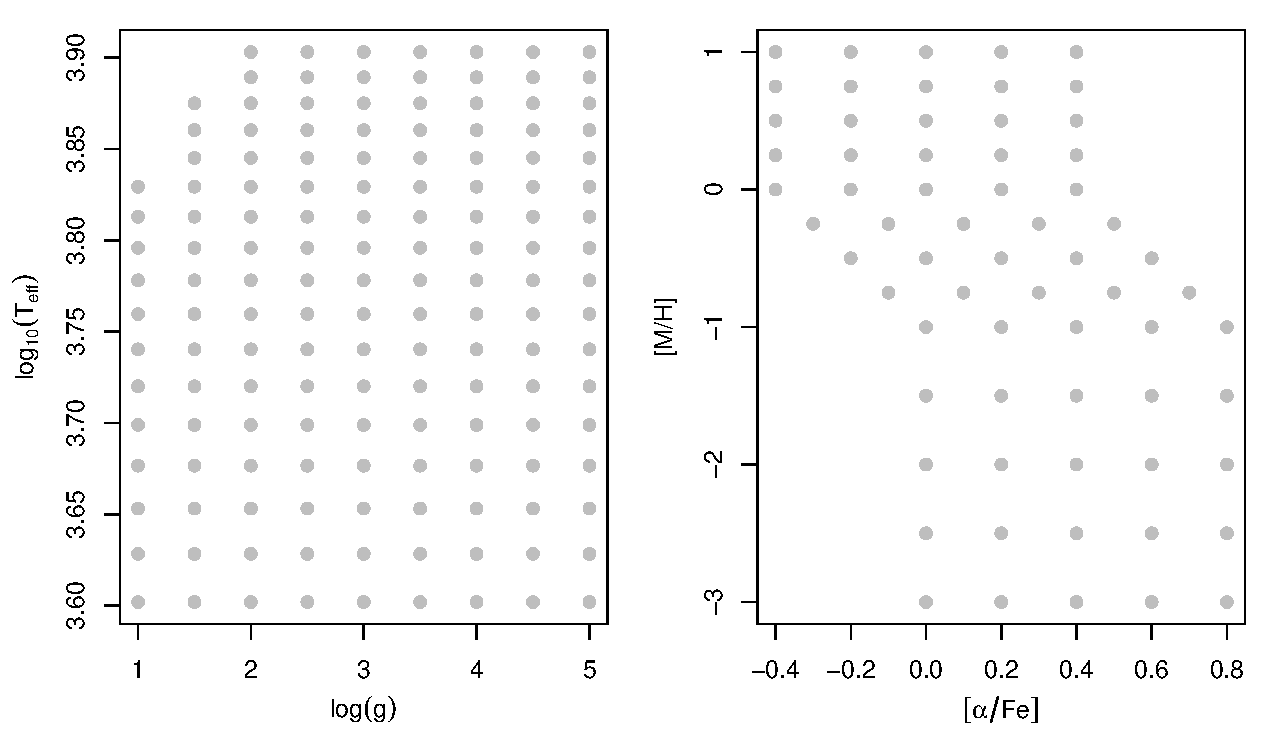
\includegraphics[width=\columnwidth]{grid_modelos.pdf}
\caption{Coverage in parameter space of the dataset}
\label{fig:gridModelos}
\end{figure}

\begin{figure*}
\centering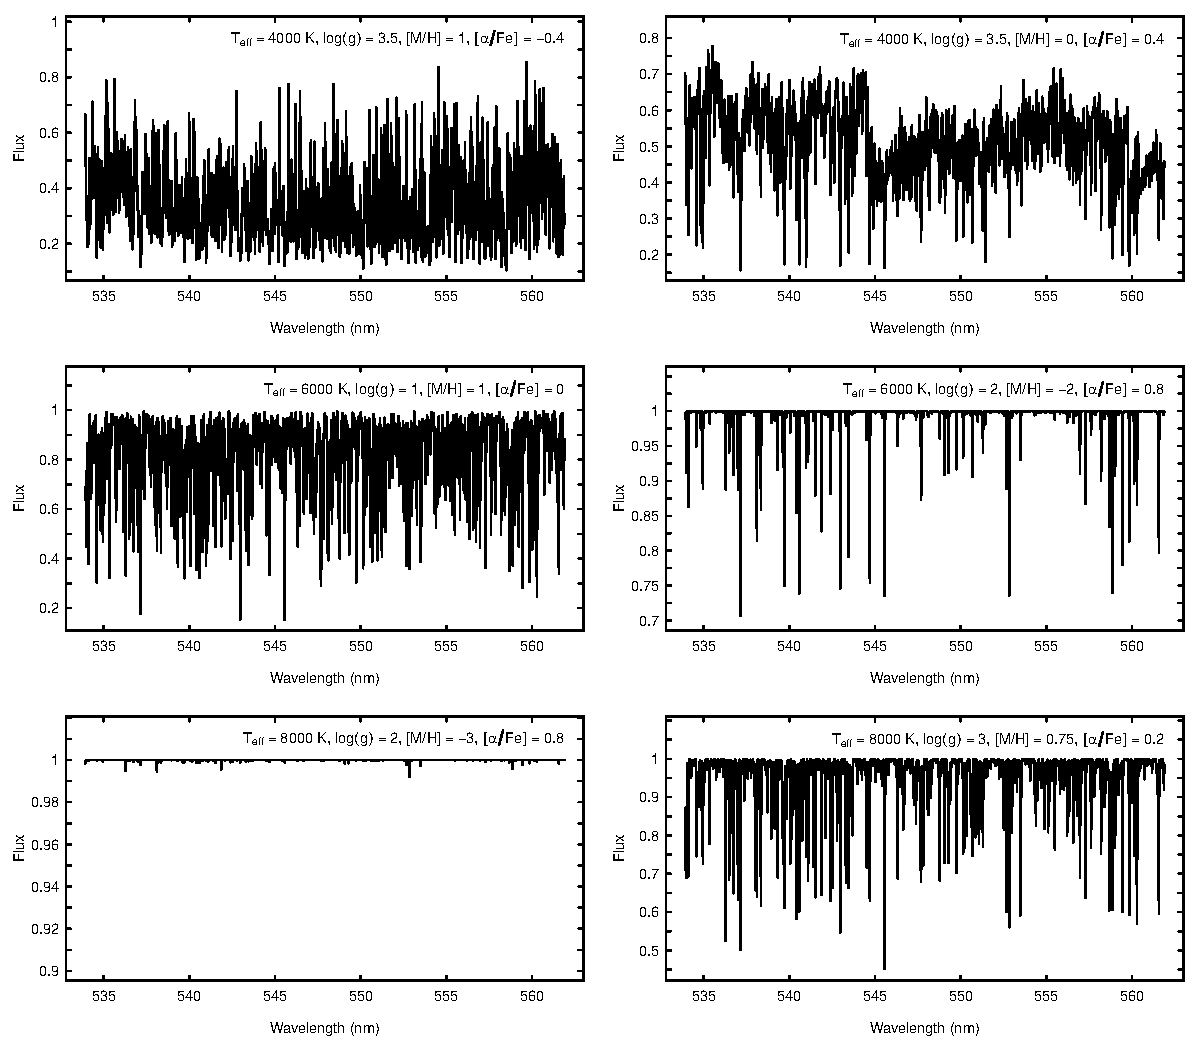
\includegraphics[width=\textwidth]{espectros.pdf}
\caption{Example spectra from the dataset}
\label{fig:ejemplosEspectros}
\end{figure*}

%The dataset contains a grid of 8780 synthetic high-resolution spectra (\textit{R} = 19800) between 5339 and 5619 {\AA} 
%% $\mathring{\mathrm{A}}$ 
%with the following parameters:
%\begin{itemize}
%\item Effective Temperature (in K): 4000-8000K, step=250K
%\item Stellar surface gravity (\textit{g} in $cm/s^2$): log \textit{g} = 1.0 - 5.0, step=0.5
%\item Mean stellar metallicity (in dex): [M/H]= -3.0 - +1.0, step=0.5 or 0.25dex
%\item $\left[ alpha/Fe \right]$ = values varying between -0.4 and +0.4dex (step=0.2dex) around the standard relation
%
%\begin{itemize}
%\item $\left[ \alpha/Fe \right]$ = +0.0dex for [M/H] $\geqslant$ 0
%\item $\left[ alpha/Fe \right]$ = +0.4dex for [M/H] $\leqslant$ -1.0
%\item $\left[ alpha/Fe \right]$ = -0.4*[M/H] for [M/H] between -1.0 and +0.0
%\end{itemize}
% Elements considered to be alpha elements are O, Ne, Mg, Si, S, Ar, Ca and Ti
%\end{itemize}

The sample size of our dataset (8780 spectra) is relatively
small compared to the input dimension (2798 flux measurements
per spectrum). For example, with an amount of information 
about 10 samples per dimension --a rule of thumb is to have at 
least 10 training samples per feature dimension \citep{jain:00}, 
the dataset should contain $10^{2798}$ spectra.
In most real case applications, the ratio of sample size to input 
dimensions is much lower and thus, the \textit{curse of dimensionality} 
problem is expected to affect even more severely the inference process. 


\subsection{The experiments}
\label{sec:modelling}

We investigate the utility of six dimensionality reduction techniques
for feature extraction with a view to improving the performance of the
estimation of atmospheric parameters. Furthermore, the robustness of
these techniques against increasing SNR is evaluated, and the
generalisation performance of training sets of varying SNRs is
analysed.

Our set of experiments proceeds in three stages: in the first
  stage we aim at selecting the compression technique and final
  dimension that minimizes the atmospheric parameter ($T_{\rm eff}$, 
  log \textit{g} or [M/H]) estimation error; in the
  second stage we analyse the estimation error for each compression
  technique as a function of the SNR of the original spectrum; and
  finally, we select the best performing compression technique and
  study the generalisation performance of an SVM model trained with
  different sets of spectra of various SNRs.

Different machine learning models have been used for the
  automatic estimation of atmospheric parameters from stellar
  spectra}. Two of the most widely used techniques in practice are
artificial neural networks (ANN) and support vector machines
(SVM). Unlike ANN, SVM does not need a choice of architecture before
training, but there are some parameters to adjust in the kernel
functions of the SVM. We use SVMs with radial basis kernel
  functions and adjust the SVM parameters by maximizing the quality of
  the  atmospheric parameter ($T_{\rm eff}$, 
  log \textit{g} or [M/H]) prediction as measured 
  by the root mean squared error (RMSE) (equation~(\ref{eq:rmse})).

\begin{equation}
\label{eq:rmse}
RMSE=\sqrt{\frac{1}{n}\sum_{i=1}^{n}\left(\hat{T}_{i}-T_{i}\right)^{2}}
\end{equation}
%\begin{equation}
%\label{eq:mae}
%MAE=\frac{1}{n}\sum_{i=1}^{n}\left|\hat{T}_{i}-T_{i}\right|
%\end{equation}
where $\hat{T}_{i}$ is the predicted atmospheric parameter ($T_{\rm eff}$, 
  log \textit{g} or [M/H]) and $T_{i}$ is the target value. 
  
The dataset was randomly split into two sets, one for training
  (66\% of the available spectra) and one for evaluation (the
  remaining 34\%), to investigate the performance of the selected
  dimensionality reduction techniques on stellar spectra. Since the
goal of these first experiments is to compare the reduction techniques
rather than obtaining the best predictor, splitting the dataset into
training and evaluation sets is considered a good scheme. In essence,
the experimental procedure consists of the following steps (Fig.~
\ref{fig:flowchart}):

\begin{enumerate}
\item Compute the low-dimensional representation of the data using the
  training set. Because some of the techniques used to reduce the 
  dimensionality depend on the setting of one or more parameters, 
  a tuning process was performed in order to determine the optimal 
  parameter values. Table~\ref{tab:parameters} presents the values 
  that were analysed in this work as well as the best parameter value 
  obtained in each case.
\item Construct SVM models based on a varying number of dimensions (2,
  5, 10, 15, 20, 25, 30 and 40) from the reduced space and the
    training set. SVM parameters (kernel size and noise contribution)
    are fine-tuned to minimize the prediction error of the 
    atmospheric parameter ($T_{\rm eff}$, log \textit{g} or [M/H]).
\item Project the evaluation set spectra onto the
  low-dimensional space computed in step 1.
\item Obtain atmospheric parameter ($T_{\rm eff}$, 
  log \textit{g} or [M/H]) estimations with the SVM models trained in step
  2 based on the new features obtained in step 3.
\item Calculate the performance of the predictor based on the RMSE
  obtained on the evaluation set.
\end{enumerate}

\begin{figure*}
\centering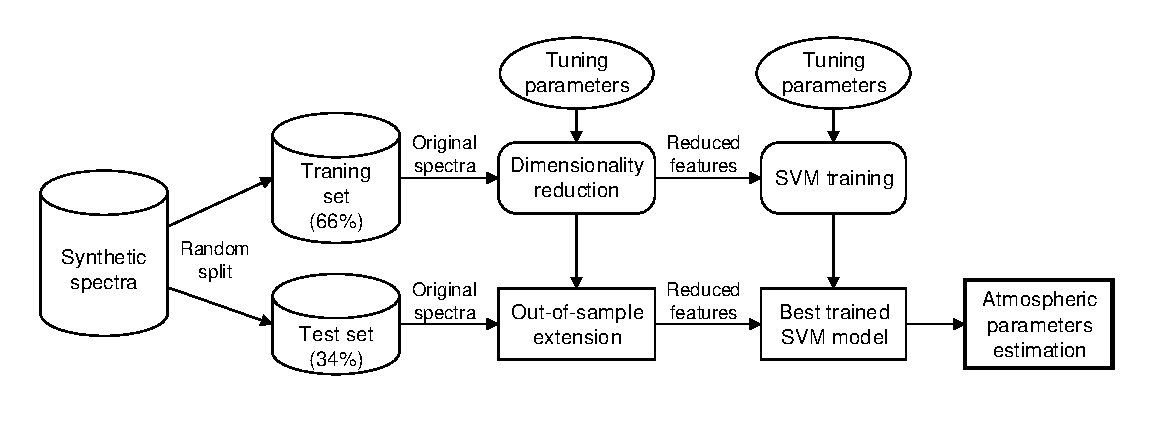
\includegraphics[width=0.8\textwidth]{flowchart.pdf}
\caption{Process flow chart for investigating the performance of the 
selected dimensionality reduction techniques.}
\label{fig:flowchart}
\end{figure*}

\begin{table}
\centering
\caption{Summary of the parameters analysed for the 
dimensionality reduction techniques.}
\label{tab:parameters}
\begin{tabular}{l c c c}
\hline
\textbf{Technique} & \textbf{Parameter} & \textbf{analysed range} & \textbf{Best value} \\
\hline
\multirow{2}{*}{DLA} 
	& $k_1$ & [2 - 8]  & 2 \\\cline{2-4}
	& $k_2$ & [2 - 8]  & 3 \\\hline
DMAP & eps.val & [0.01 - 700] & 600 \\\hline
KPCA & $\sigma$ & [0.0001 - 0.01] & 0.001 \\
\hline
\end{tabular}
\end{table}


The same procedure described above was used to analyse the 
  robustness properties of the selected dimensionality reduction
techniques against increasing noise rates. In this case,
Gaussian white noise of different variances (SNR equal to 100,
50, 25 and 10) was added to the original synthetic spectra.
 
The optimal compression method and the optimal reduced
  dimension were selected according to the results of the previous
  experiments to investigate the optimal SNR of the training samples
  with a view to obtaining the best generalization performance of the
  atmospheric parameters estimators. Twenty-five datasets were
  generated for a wider range of SNR levels (150, 125, 100, 75, 50,
  25, 10 and 5) and SVM models were trained to estimate the atmospheric 
  parameter ($T_{\rm eff}$, log \textit{g} or [M/H]) to
  assess the consistency of the results. Each SVM model was used to
  estimate the atmospheric parameters ($T_{\rm eff}$, 
  log \textit{g} or [M/H]) for spectra with SNR ratios different from
  those used during the learning phase.  The performance measure of
  the models was evaluated using 10-fold cross validation:

\begin{enumerate}
\item The dataset was split into 10 smaller sets or \textit{folds}.
\item The optimal compression technique was applied to nine of
  the these folds, and the original spectra compressed to a space
  of the dimensionality found optimal in the experiments described in
  previous paragraphs.
\item A SVM model was trained using the training spectra projected
  onto the new space.
\item The tenth fold was used as the evaluation set. The spectra
  were projected onto the new low-dimensional space and the
    SVM model used to estimate the corresponding  atmospheric parameter 
    ($T_{\rm eff}$, log \textit{g} or [M/H]). Then the
  quality of the prediction was measured.
\item Step 4 was repeated using spectra with different SNR to that
  used for computing the ICA projector and for training the SVM model.
\item Steps 2 to 5 were repeated 10 times (using each time a
  different fold for evaluation) and the performance measure was
  calculated by averaging the values obtained in the loop.
\end{enumerate}

Finally, an analysis of the effect of the grid density over the 
performance in atmospheric parameters estimation was carried out. 
To do this, six new datasets of synthetic spectra were computed
by considering different grid densities. Thus, the $T_{\rm eff}$ 
values varied between 4000 and 8000 K with a variable step-size 
between 50 K and 250 K. The other grid parameters were established 
as follows: the log \textit{g} were regularly sampled from 1 to 5 
in 0.5 steps and both [M/H] and $\left[ \alpha/Fe \right]$ were 
equal zero. Table~\ref{tab:grid} presents the step-sizes used in this 
study as well as the number of synthetic spectra available in each grid.
Furthermore, different SNR levels (100, 50, 25, 10) were added to
the original synthetic spectra.

\begin{table}
\centering
\caption{Size of the new datasets computed with different grid densities.}
\label{tab:grid}
\begin{tabular}{c c}
\hline
\textbf{$T_{\rm eff}$ step-size (K)} & \textbf{Number of spectra} \\
\hline
50 & 679 \\
62.5 & 545 \\
100 & 343 \\
125 & 277 \\
200 & 175\\
250 & 143\\
\hline
\end{tabular}
\end{table}

The performance of the $T_{\rm eff}$ models trained with the new 
datasets was evaluated using 10-fold cross validation.

\section{Results and discussion}
\label{sec:results}
In this section, we present the results of the experiments 
  described in the Sect. \ref{sec:experiment}.

First, we compare the performance of the dimensionality reduction
techniques described in section \ref{sec:dimred} using noise-free
synthetic spectra as well as degraded spectra with SNR levels of 100,
50, 25 and 10.  Fig.~\ref{fig:01} to \ref{fig:06} show the
RMSE obtained with the evaluation set (the 34\% of the full set of
spectra that was not not used to define the compression transformation
or to train SVM models). Overall, wavelets combined with SVM
models have the highest errors regardless of the number of retained
dimensions, with the exception of [M/H] estimation where DLA performed 
worse for noisy synthetic spectra. DLA achieved the lowest prediction 
errors for the unrealistic noise-free data. Furthermore, the performance 
of this technique was the best for the highest compression rates 
(two or five dimensions) to estimate $T_{\rm eff}$ and 
log \textit{g}. However, it was outperformed by the other techniques 
in almost any other case. PCA and diffusion maps yielded similar 
prediction errors in $T_{\rm eff}$ estimation. As for the estimation 
of surface gravity and metallicity, results obtained with PCA 
were better than results from diffusion maps. An important 
characteristic of diffusion maps combined with SVM models is that 
similar estimation errors were obtained regardless of the SNR of 
the data.

Finally, the best strategies to compress the spectra are kernel PCA 
and ICA, with ICA outperforming kernel PCA in most of the parameter
space. RMSE errors increased only moderately down to a SNR of 10
which seems to indicate that most of the examined compression
techniques serve well as noise filters.

The performance comparison of the analysed dimensionality reduction
techniques shows that although traditional PCA is not the most
efficient method, it outperforms some of the nonlinear techniques used
in this study, such as diffusion maps, DLA or wavelets.

\begin{figure}
\centering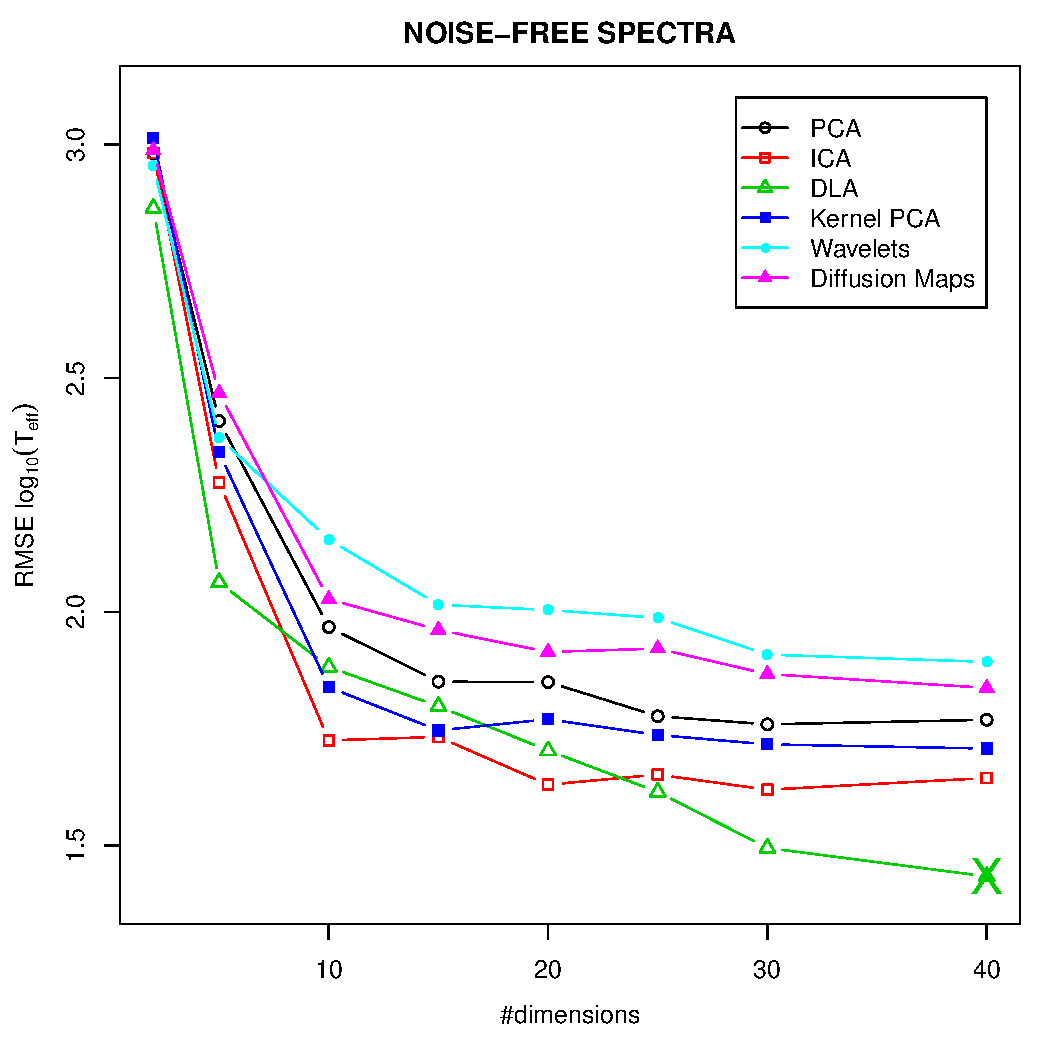
\includegraphics[width=\columnwidth]{flamesHR10_SNR=000_Teff_log_BestSVM_N-RMSE_test.pdf}
\caption{Temperature estimation error as a function of the number of
  dimensions used for data compression, for synthetic spectra}
\label{fig:01}
\end{figure}

\begin{figure*}
\centering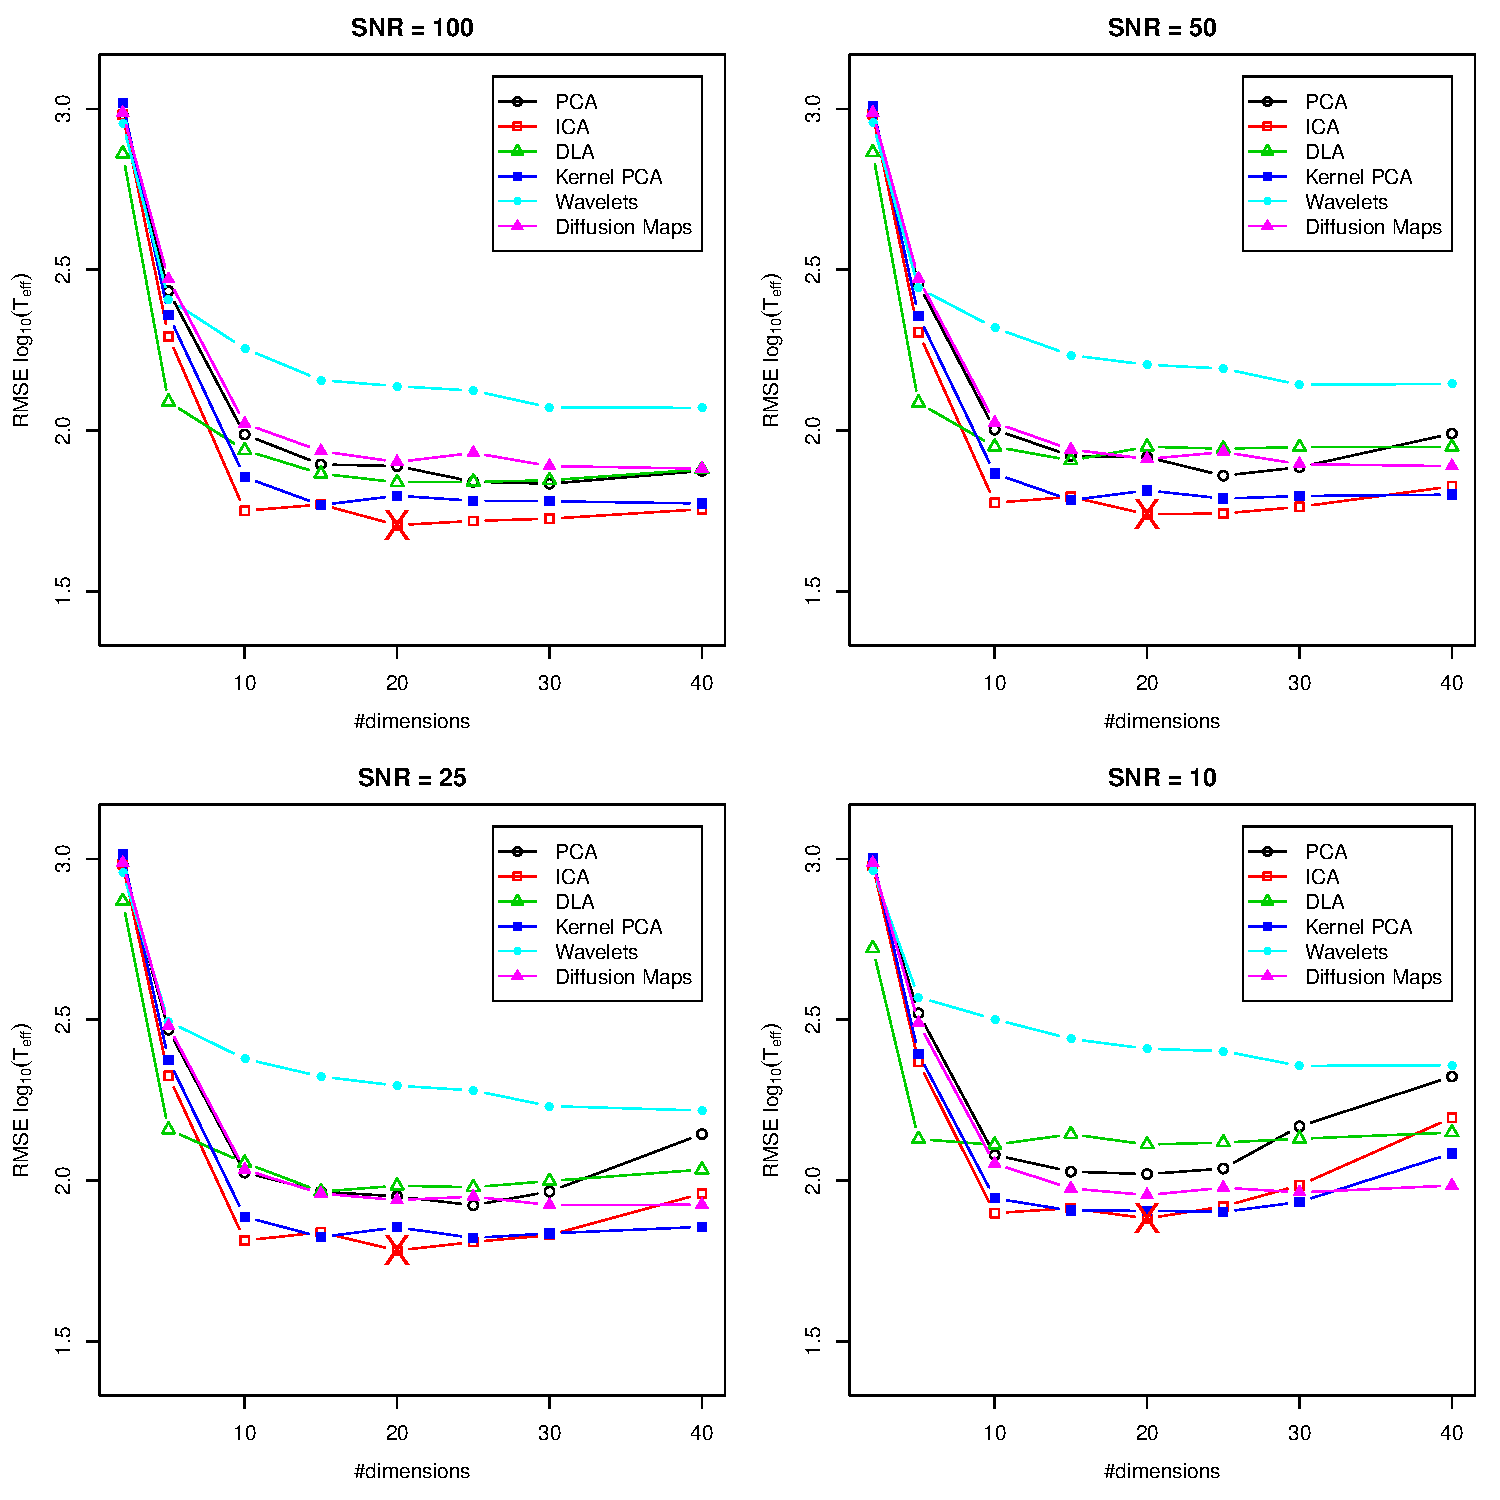
\includegraphics[width=\textwidth]{flamesHR10_Teff_log_BestSVM_N-RMSE_test.pdf}
\caption{Temperature estimation error as a function of the number of
  dimensions used for data compression, for noisy synthetic
  spectra.}
\label{fig:02}
\end{figure*}

\begin{figure}
\centering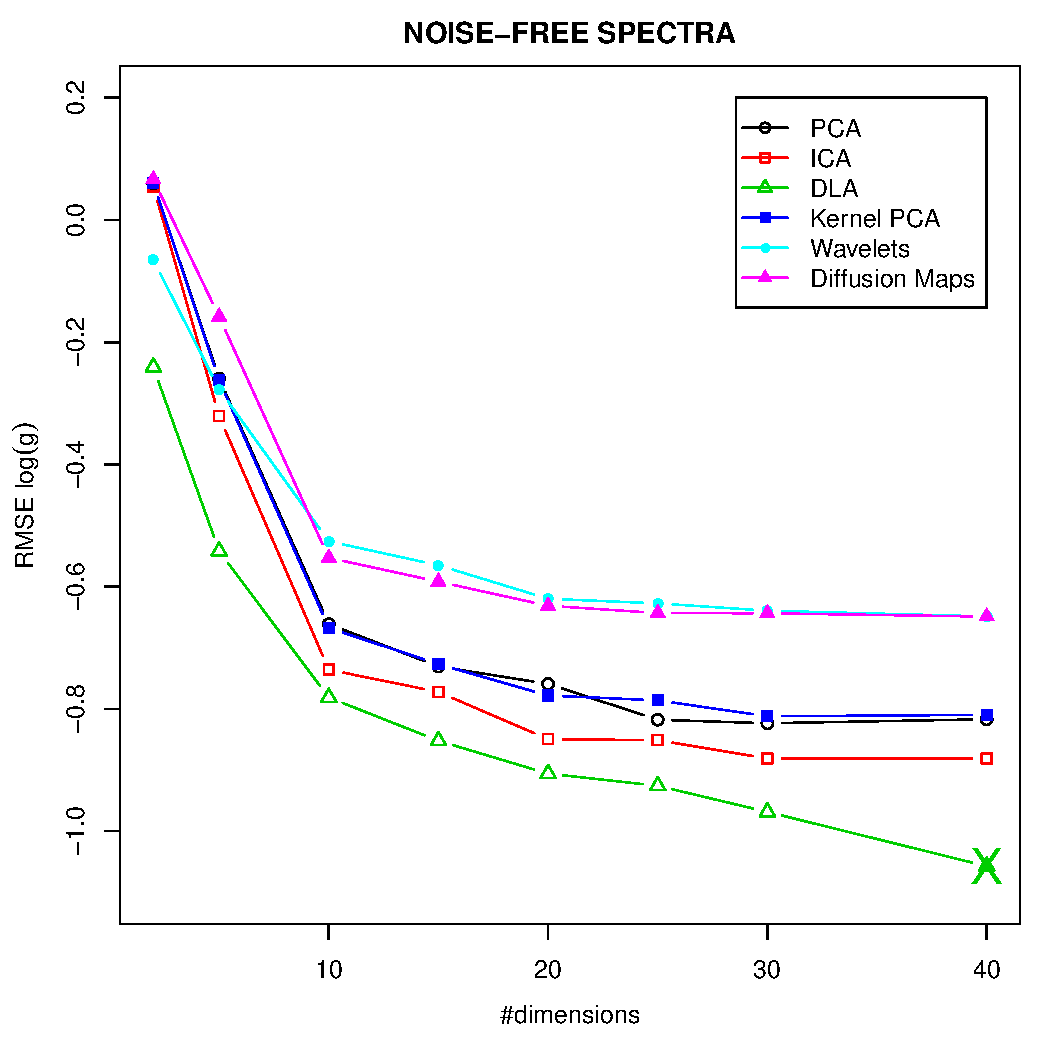
\includegraphics[width=\columnwidth]{flamesHR10_SNR=000_Logg_log_BestSVM_N-RMSE_test.pdf}
\caption{Surface gravity estimation error as a function of the number of
  dimensions used for data compression, for synthetic spectra}
\label{fig:03}
\end{figure}

\begin{figure*}
\centering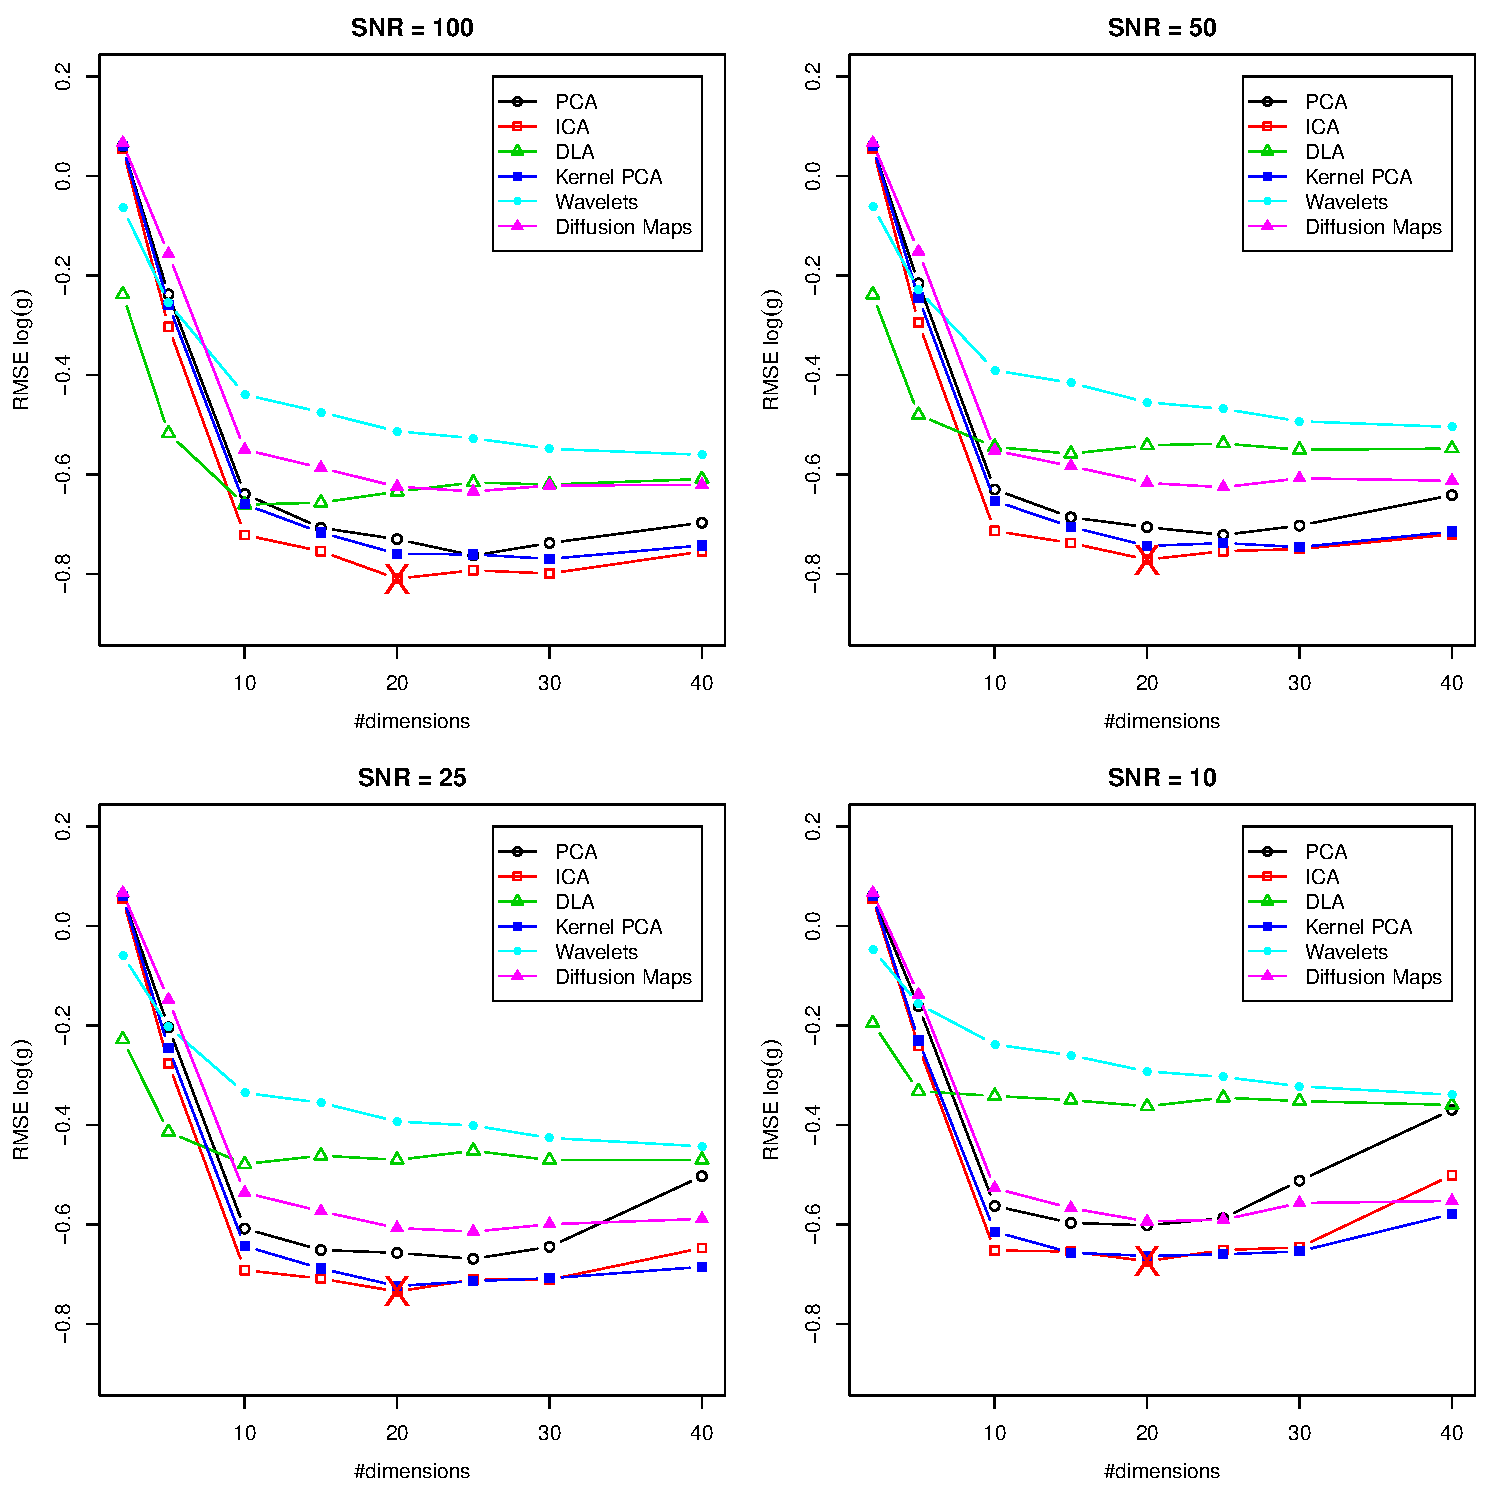
\includegraphics[width=\textwidth]{flamesHR10_Logg_log_BestSVM_N-RMSE_test.pdf}
\caption{Surface gravity estimation error as a function of the number of
  dimensions used for data compression, for noisy synthetic
  spectra.}
\label{fig:04}
\end{figure*}

\begin{figure}
\centering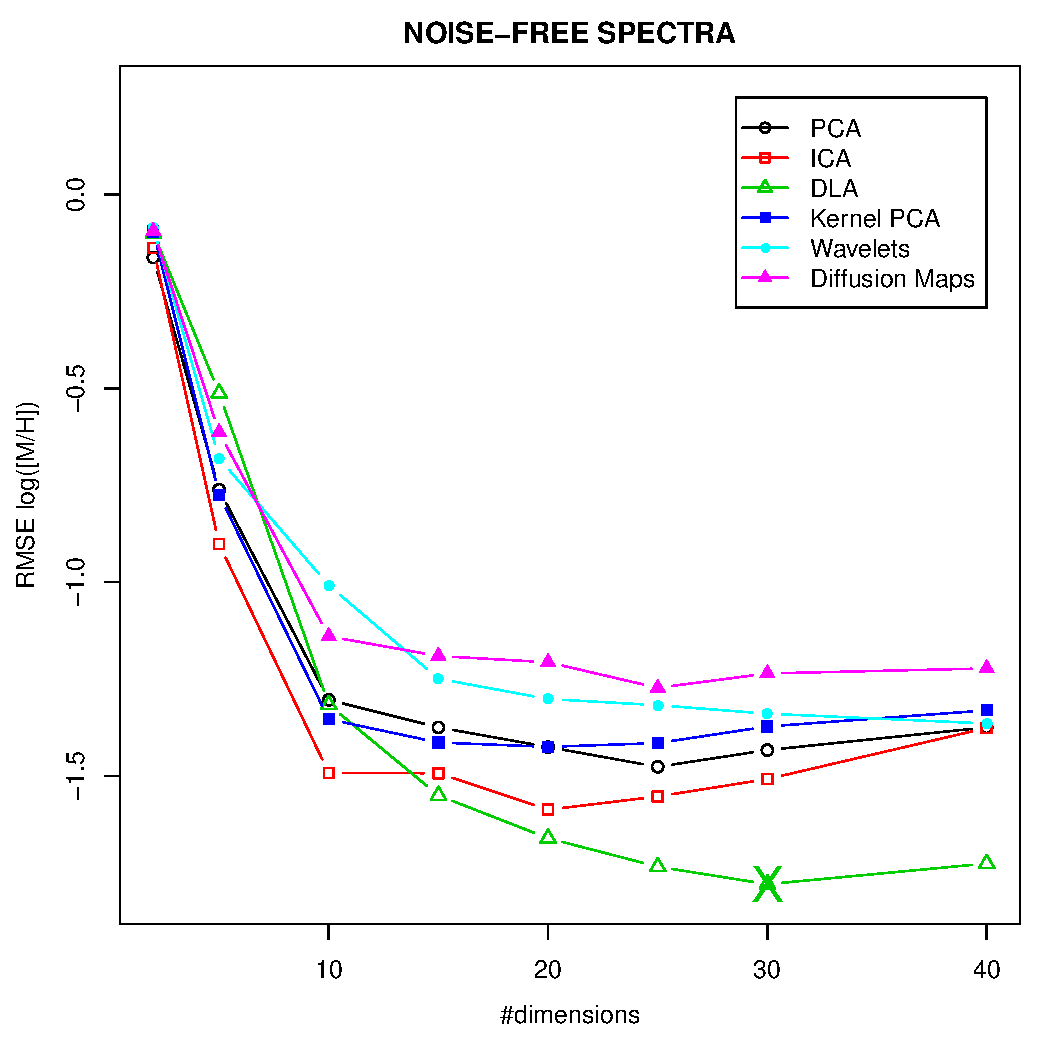
\includegraphics[width=\columnwidth]{flamesHR10_SNR=000_Meta_log_BestSVM_N-RMSE_test.pdf}
\caption{Metallicity estimation error as a function of the number of
  dimensions used for data compression, for synthetic spectra}
\label{fig:05}
\end{figure}

\begin{figure*}
\centering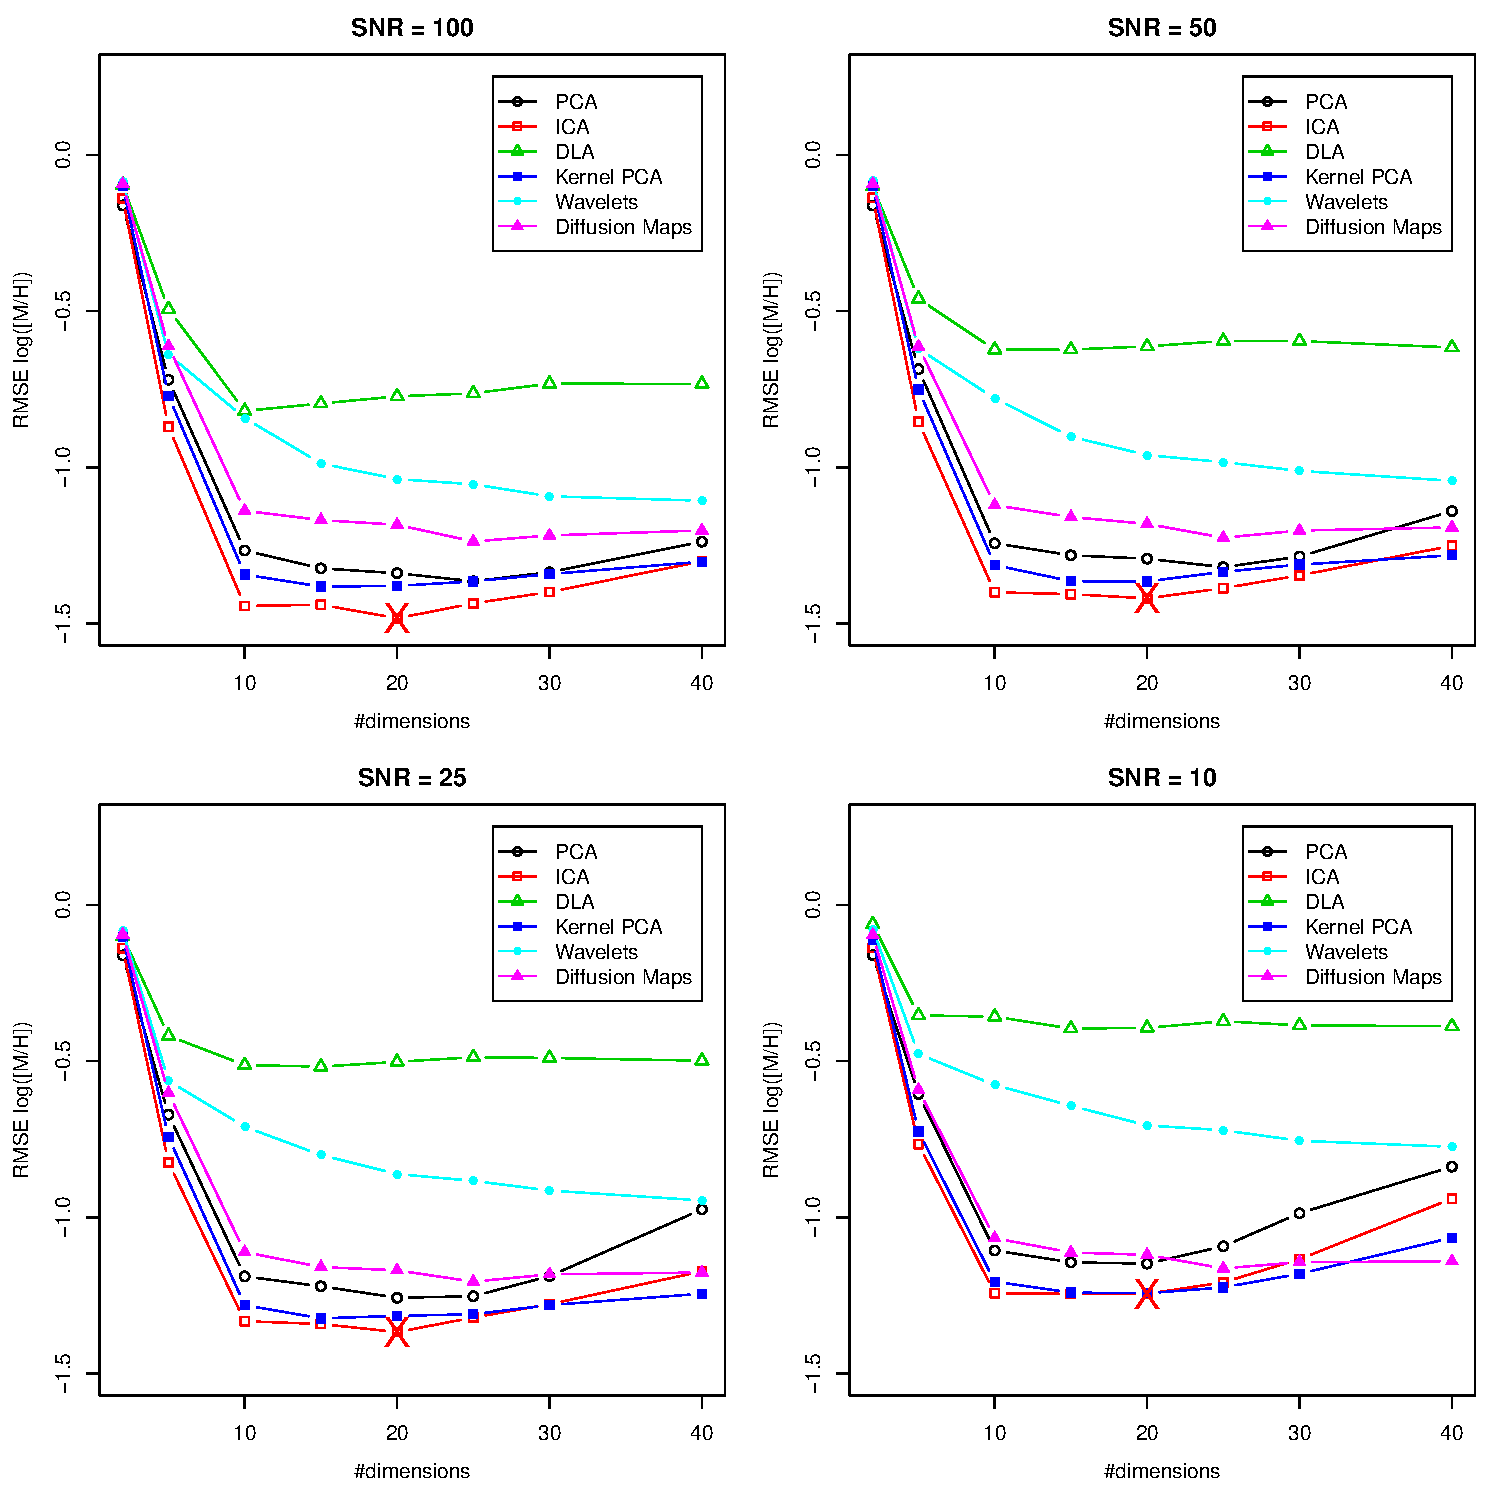
\includegraphics[width=\textwidth]{flamesHR10_Meta_log_BestSVM_N-RMSE_test.pdf}
\caption{Metallicity estimation error as a function of the number of
  dimensions used for data compression, for noisy synthetic
  spectra.}
\label{fig:06}
\end{figure*}

Table~\ref{tab:01} quantifies the prediction errors of the best models
trained for each SNR. It is interesting that ICA compression with 20
independent components remains as the best option for any SNR, except
for the unrealistic noise-free data. These results evidence that
for a given sample size (the number of spectra in this particular 
application)
there is an optimal number of features beyond which the
performance of the predictor will degrade rather than improve. 
On the other hand, as expected, the quality of atmospheric parameter 
($T_{\rm eff}$, log \textit{g} or [M/H]) predictions 
  degrades for lower SNR (see Fig.~\ref{fig:methodsnrTeff}, 
  \ref{fig:methodsnrLogg} and \ref{fig:methodsnrMeta}). However,
RMSE errors were relatively low even for low SNR ($\sim$ 10).
It is worth mentioning that diffusion maps and kernel PCA give 
quite stable results regardless of the SNR of the spectra.


\begin{table*}
\centering
\caption{RMSE on the evaluation set of 2986 spectra for the best SVM trained models.}
\label{tab:01}
\resizebox{0.99\textwidth}{!}{%
\begin{tabular}{l c c c c c}
\hline
\textbf{SNR} & \textbf{Method} & \textbf{Dimension} & \textbf{$RMSE (T_{\rm eff}, K)$} & \textbf{$RMSE (log \textit{g})$} & \textbf{$RMSE ([M/H], dex)$}\\
\hline
Noise-free & DLA & 40 / 30$^1$ & 27.16 & 0.13 & 0.017\\
100 & ICA & 20 & 50.81 & 0.15 & 0.033\\
50 & ICA & 20 & 54.91 & 0.17 & 0.038\\
25 & ICA & 20 & 60.59 & 0.18 & 0.043\\
10 & ICA & 20 & 76.21 & 0.21 & 0.057\\
\hline
\multicolumn{6}{l}{$^1$ The best performance for [M/H]  
was obtained with 30 dimensions instead of 40.}\\
\end{tabular}
}
\end{table*}

%\begin{table}[h]
%\centering
%\begin{tabular}{l c c c c}
%\hline
%\textbf{SNR} & \textbf{Method} & \textbf{Dimension} & \textbf{$RMSE (T_{eff}, K)$} & \textbf{$MAE (T_{eff}, K)$}\\
%\hline
%Noise-free data & DLA & 40 & 27.16 & 8.37 \\
%100 & ICA & 20 & 50.81 & 28.24 \\
%50 & ICA & 20 & 54.91 & 34.75 \\
%25 & ICA & 20 & 60.59 & 37.57 \\
%10 & ICA & 20 & 76.21 & 53.48 \\
%\hline
%\end{tabular}
%\caption{RMSE and MAE on the evaluation set of 2986 spectra for the best SVM trained models.}
%\label{tab:01}
%\end{table}

\begin{figure*}
\centering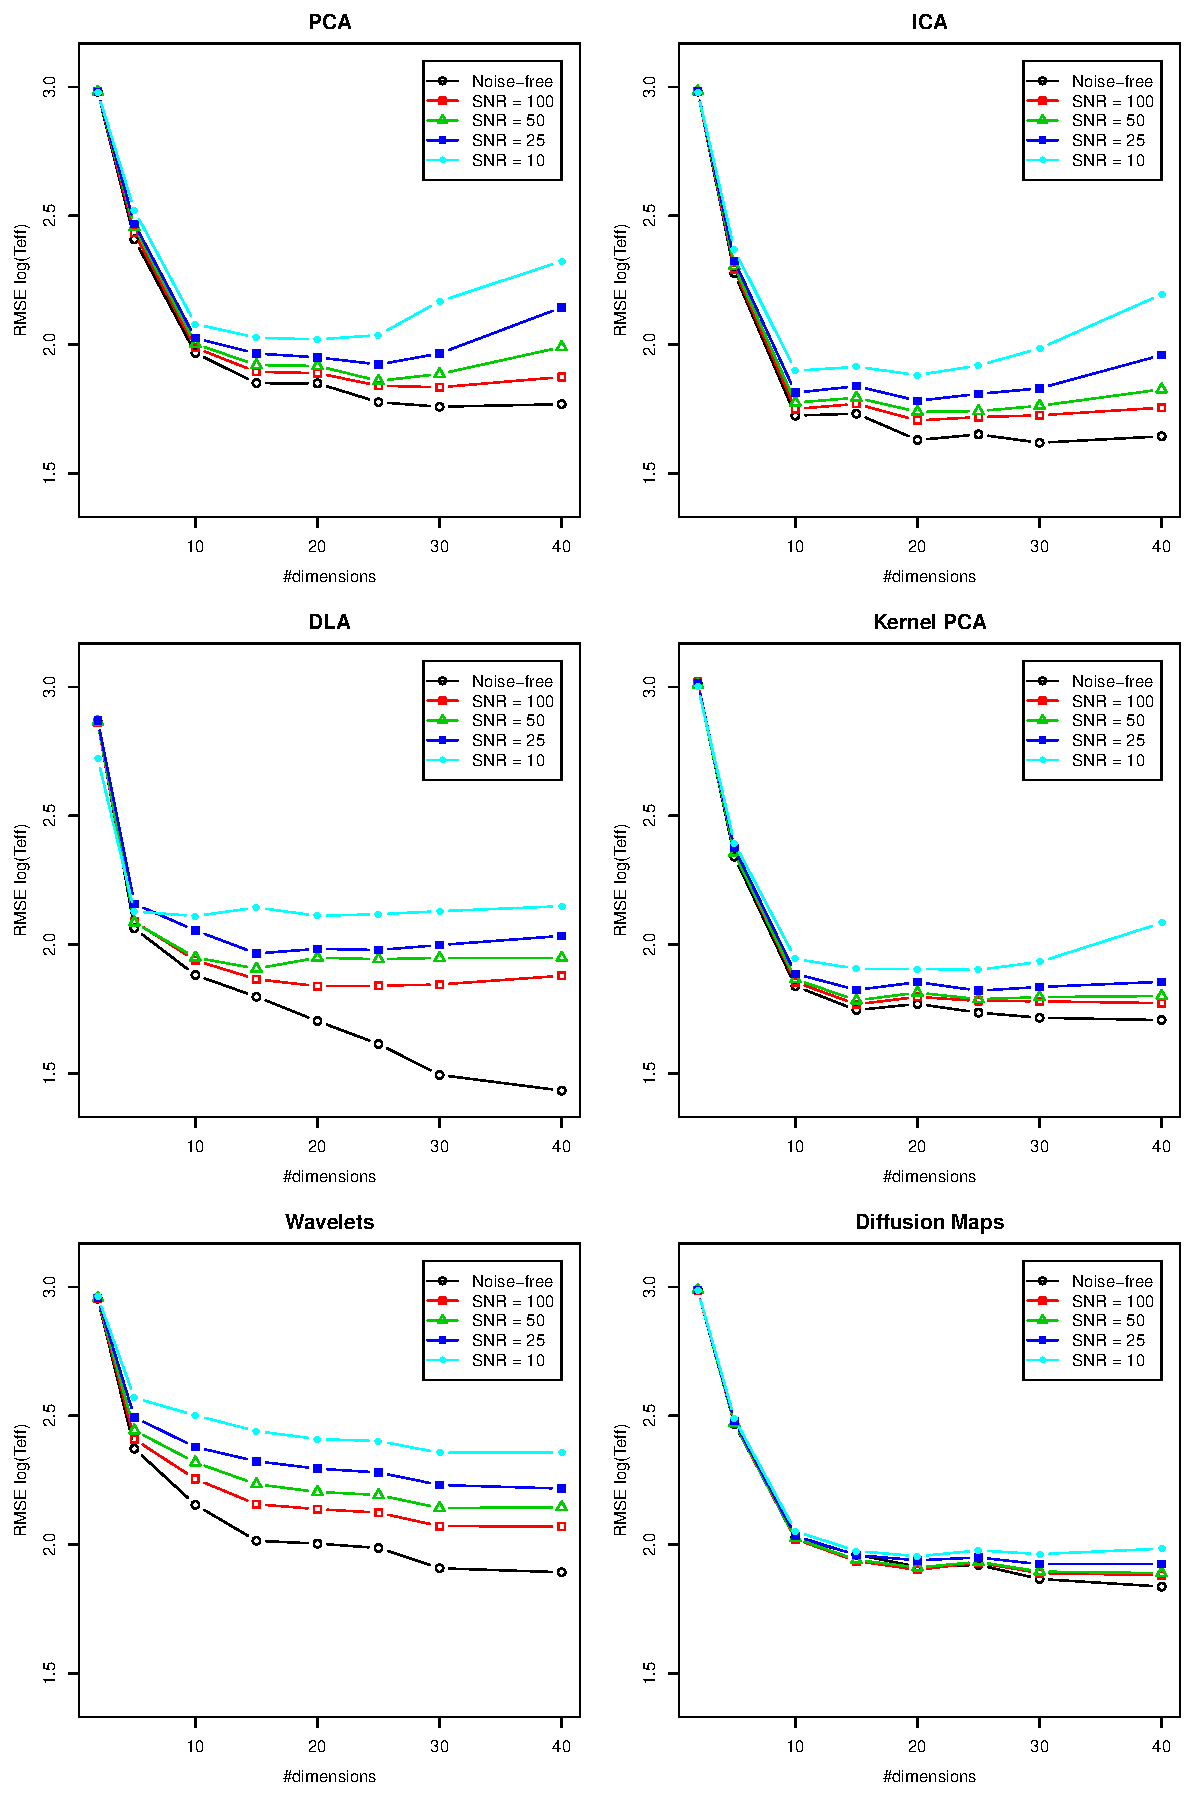
\includegraphics[height=0.95\textheight]{flamesHR10_Teff_log_BestSVM_N-SNR-RMSE_test.pdf}
\caption{Temperature estimation error against the number of dimensions
  used for data compression. Each line corresponds to a model trained
  with a specific SNR}
\label{fig:methodsnrTeff}
\end{figure*}

\begin{figure*}
\centering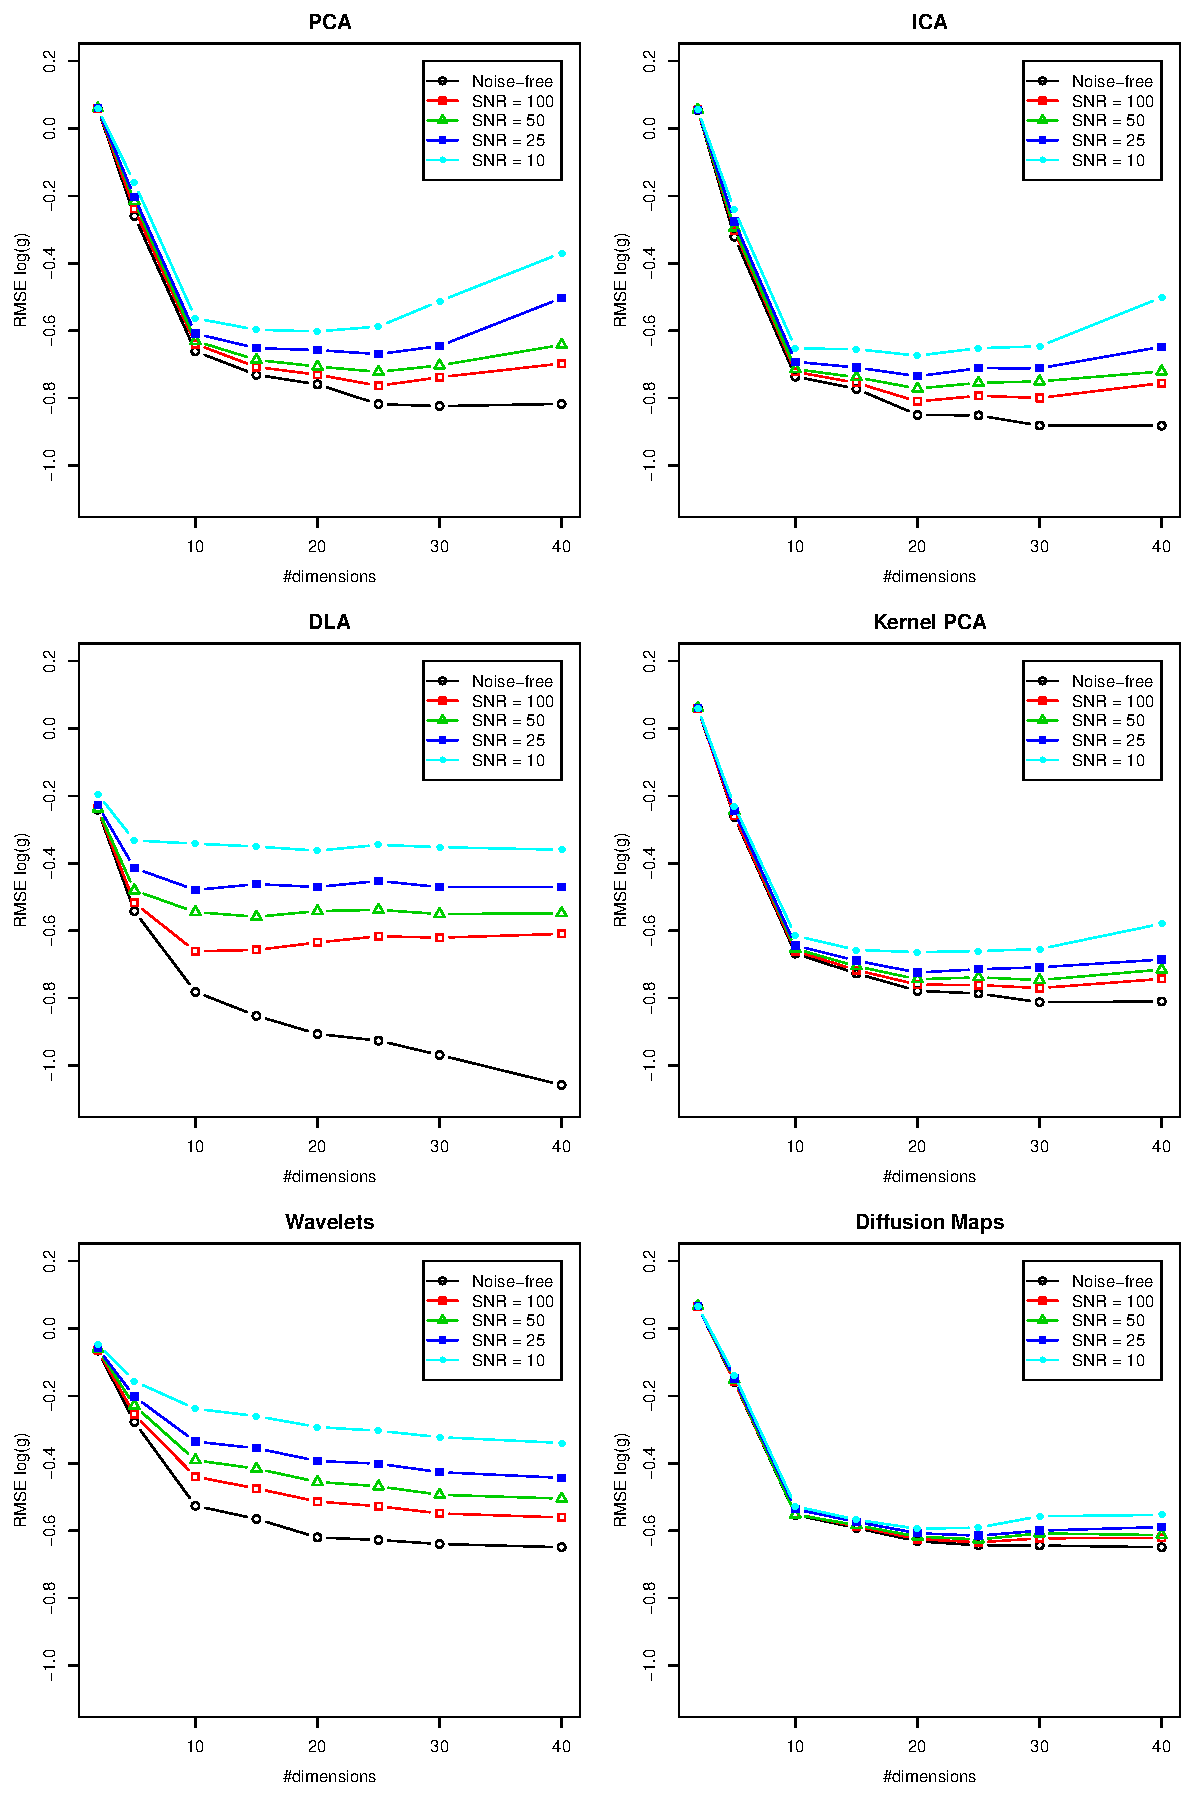
\includegraphics[height=0.95\textheight]{flamesHR10_Logg_log_BestSVM_N-SNR-RMSE_test.pdf}
\caption{Surface gravity estimation error against the number of dimensions
  used for data compression. Each line corresponds to a model trained
  with a specific SNR}
\label{fig:methodsnrLogg}
\end{figure*}

\begin{figure*}
\centering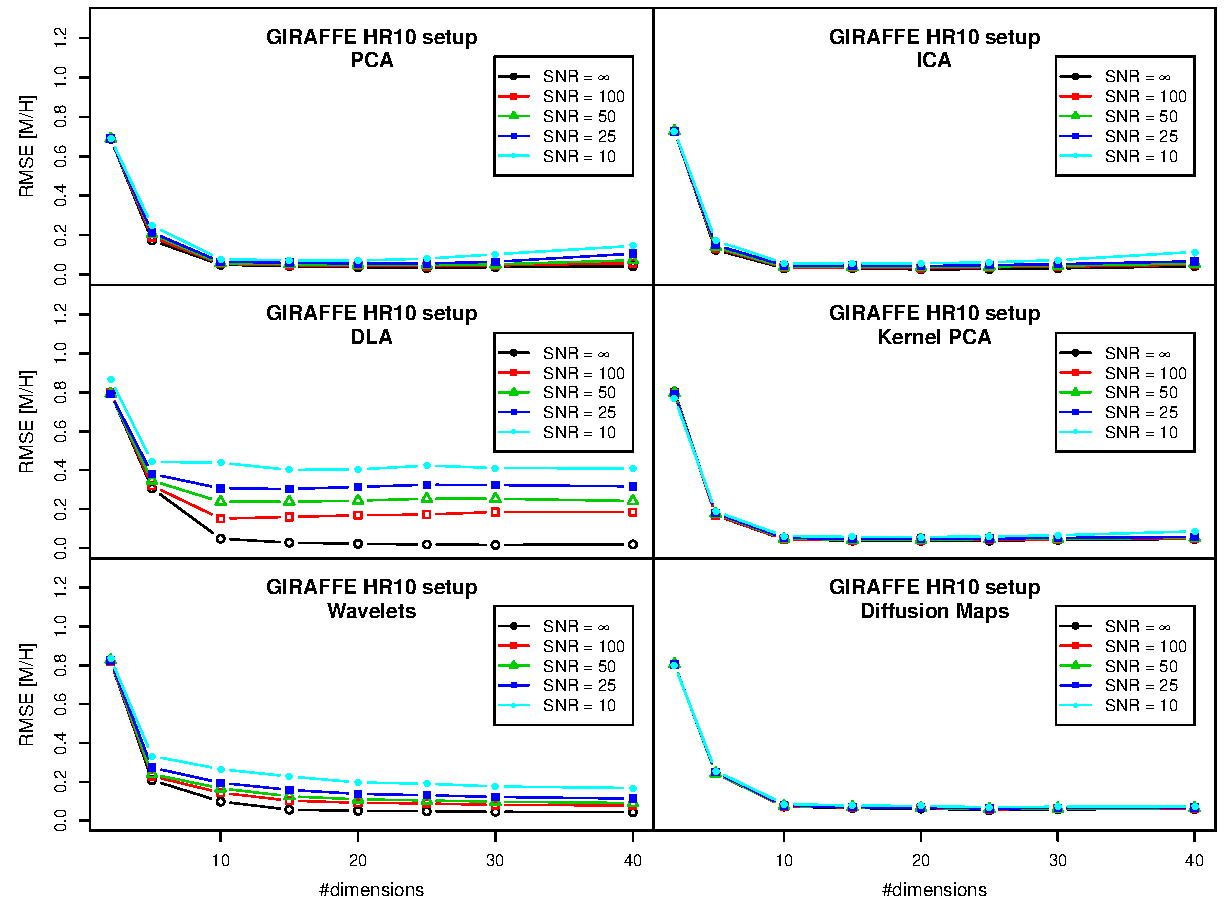
\includegraphics[height=0.95\textheight]{flamesHR10_Meta_log_BestSVM_N-SNR-RMSE_test.pdf}
\caption{Metallicity estimation error against the number of dimensions
  used for data compression. Each line corresponds to a model trained
  with a specific SNR}
\label{fig:methodsnrMeta}
\end{figure*}

According to the results shown above, the best performing
dimensionality reduction technique was ICA with 20 independent
components. Thus, we selected
this compression method to investigate the noise properties of
  the training set in order to obtain the best generalization
performance of the $T_{\rm eff}$, log \textit{g} and [M/H]
estimators.  As described in section \ref{sec:modelling}, these
experiments were carried out using 25 different noise
  realisations for each SNR analysed (150, 125, 100, 75, 50, 25, 10
and 5) in order to assess the consistency of the results.  Fig.~
\ref{fig:snrtrain} shows mean RMSE results and the 95\% confidence
interval for the mean as a function of the SNR of the evaluation
set. The nine different lines correspond to the SNR of the
training set used to generate both the projector and the atmospheric 
parameter ($T_{\rm eff}$, log \textit{g} and [M/H]) predictor. 
Main conclusions of the analysis of this figure are the
following:

\begin{itemize}
\item There are no large discrepancies amongst the estimations 
	obtained applying the same model to different datasets.
\item For spectra of SNR of about 100 or greater, there are minimal
  differences in the precision achieved with models trained with
  spectra of SNR of 50 or greater.
\item The accuracy is exponentially reduced for estimators
  constructed from noise-free spectra when the SNR of the spectra is
  about 75 or lower.
\item The overall performance is very similar when the SNR of the
  evaluation spectra is between 50 and 75, except for the noise-free
  model in the estimation of $T_{\rm eff}$. 
\item For the evaluation sets with SNR values of 25, the best accuracy
  is obtained with the model constructed from spectra with SNR of 50. 
  In the prediction of log \textit{g}, the best model corresponds to 
  that trained with SNR of 25.
\item For SNR lower than 10, the model with best generalization
  performance is that trained with SNR equal to 10 for $T_{\rm eff}$ 
  and [M/H]. The lowest prediction errors for log \textit{g} estimation 
  were obtained with the model trained with SNR equal to 25.
\end{itemize}

\begin{figure}
\centering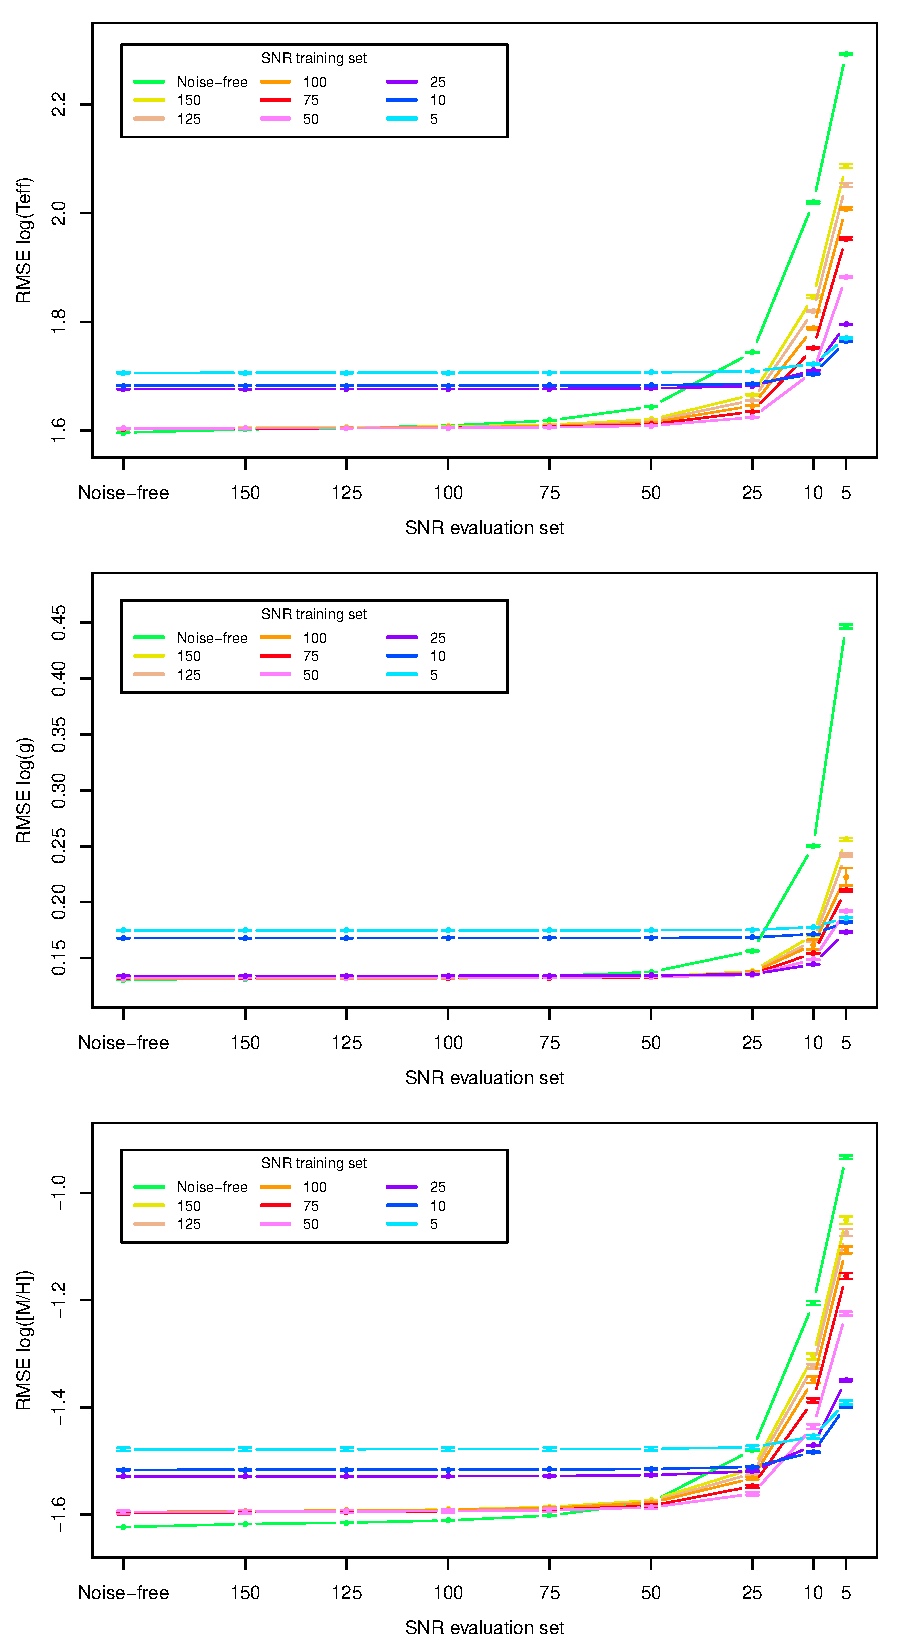
\includegraphics[width=\columnwidth]{snr_errors_log_global.pdf}
\caption{Temperature estimation error against the SNR of the evaluation set. Each line corresponds to a model trained with a specific SNR}
\label{fig:snrtrain}
\end{figure}

This analysis yields the very important consequence that models
trained with noise-free spectra are not adequate to estimate
atmospheric parameters of spectra with relatively high SNRs (up to
75). Moreover, in order to improve the generalization performance of
the models, there is no need to match the SNR of the training set to
that of the real spectra. Based on this results, two ICA+SVM models
would be enough to estimate $T_{\rm eff}$ and [M/H]: one for spectra 
with SNR of about 25 or greater (model trained with SNR of 50) and 
one for spectra with SNR of 10 or lower (model trained with SNR of 10).
On the contrary, only one ICA+SVM model trained with SNR of 25 would 
be enough to estimate the surface gravity.

Finally, Fig.~\ref{fig:gridpure} to \ref{fig:grid10} present the
$T_{\rm eff}$ estimation errors that were obtained with different 
grid densities and SNR levels. Main conclusions of the analysis 
of these figures are the following:

\begin{itemize}
\item As expected, estimation errors increase when the grid 
	density decreases.
\item Overall, the accuracy obtained against the grid density 
	is more variable when the number of dimensions retained 
	increases. 
\item PCA and ICA show a similar behaviour to the grid density 
	variation. 
\item The grid density appeared to have less effect over the 
	performance of Wavelets and diffusion maps.
\end{itemize}


\begin{figure*}
\centering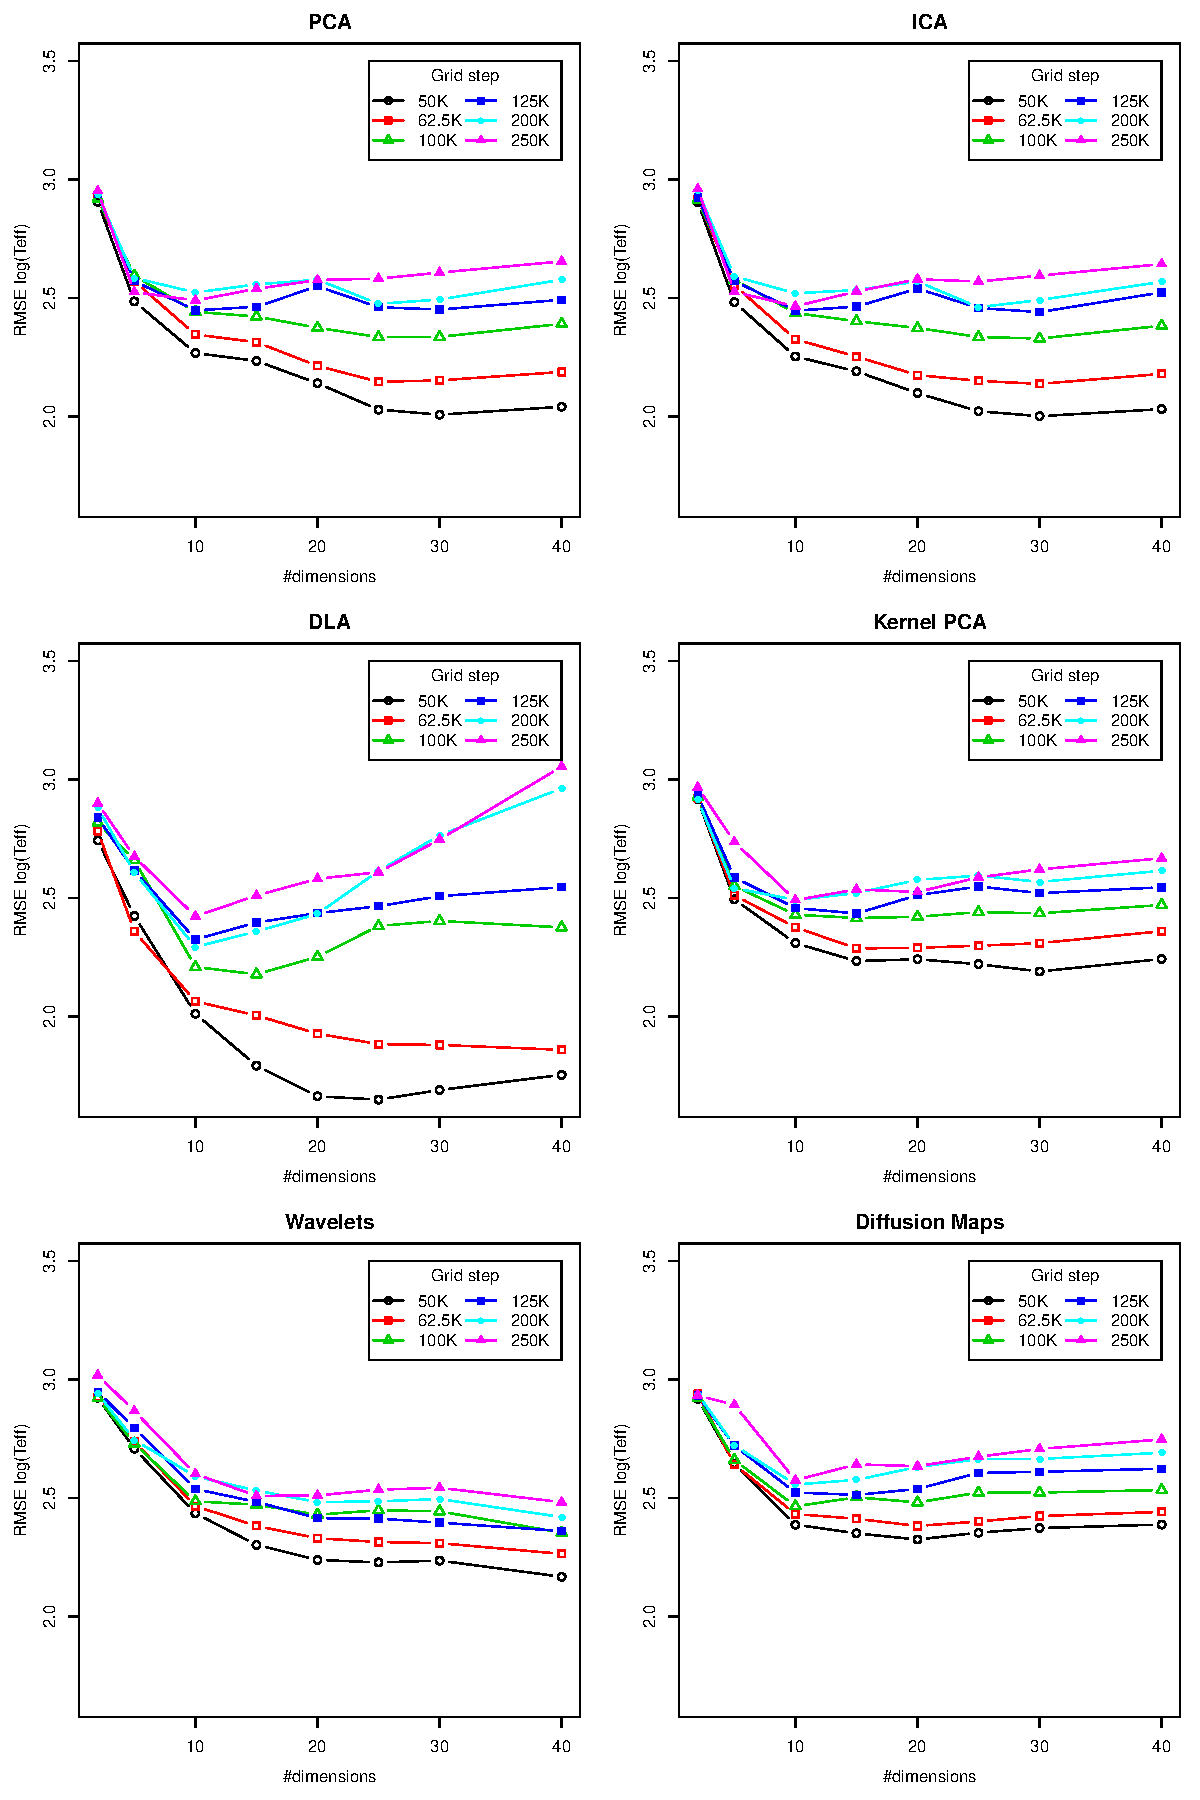
\includegraphics[height=0.95\textheight]{bestSVM_Teff_N-RMSE_HR10_pure_all.pdf}
\caption{Temperature estimation error against the number of dimensions
  used for data compression. Each line corresponds to a model trained
  with a specific grid step (Noise-free spectra)}
\label{fig:gridpure}
\end{figure*}

\begin{figure*}
\centering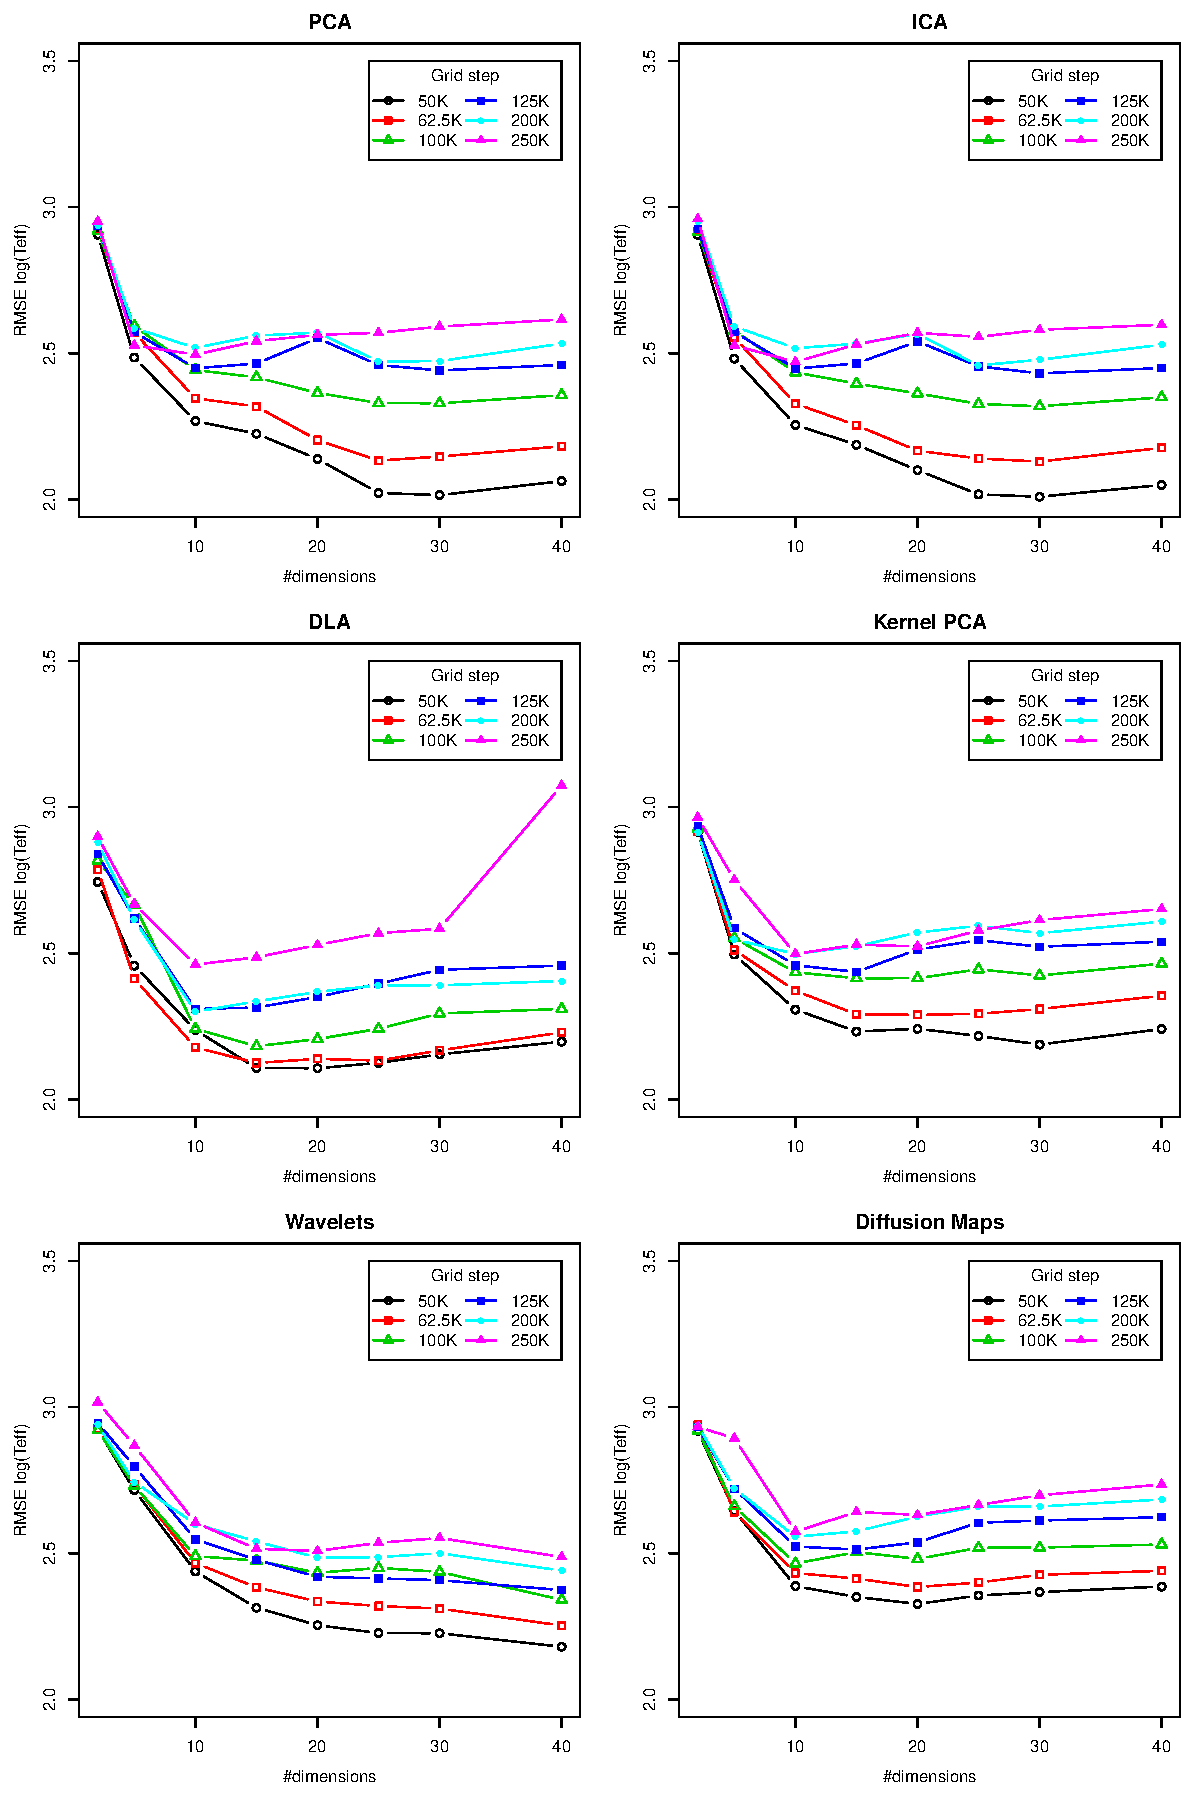
\includegraphics[height=0.95\textheight]{bestSVM_Teff_N-RMSE_HR10_snr=100_all.pdf}
\caption{Temperature estimation error against the number of dimensions
  used for data compression. Each line corresponds to a model trained
  with a specific grid step (SNR = 100)}
\label{fig:grid100}
\end{figure*}

\begin{figure*}
\centering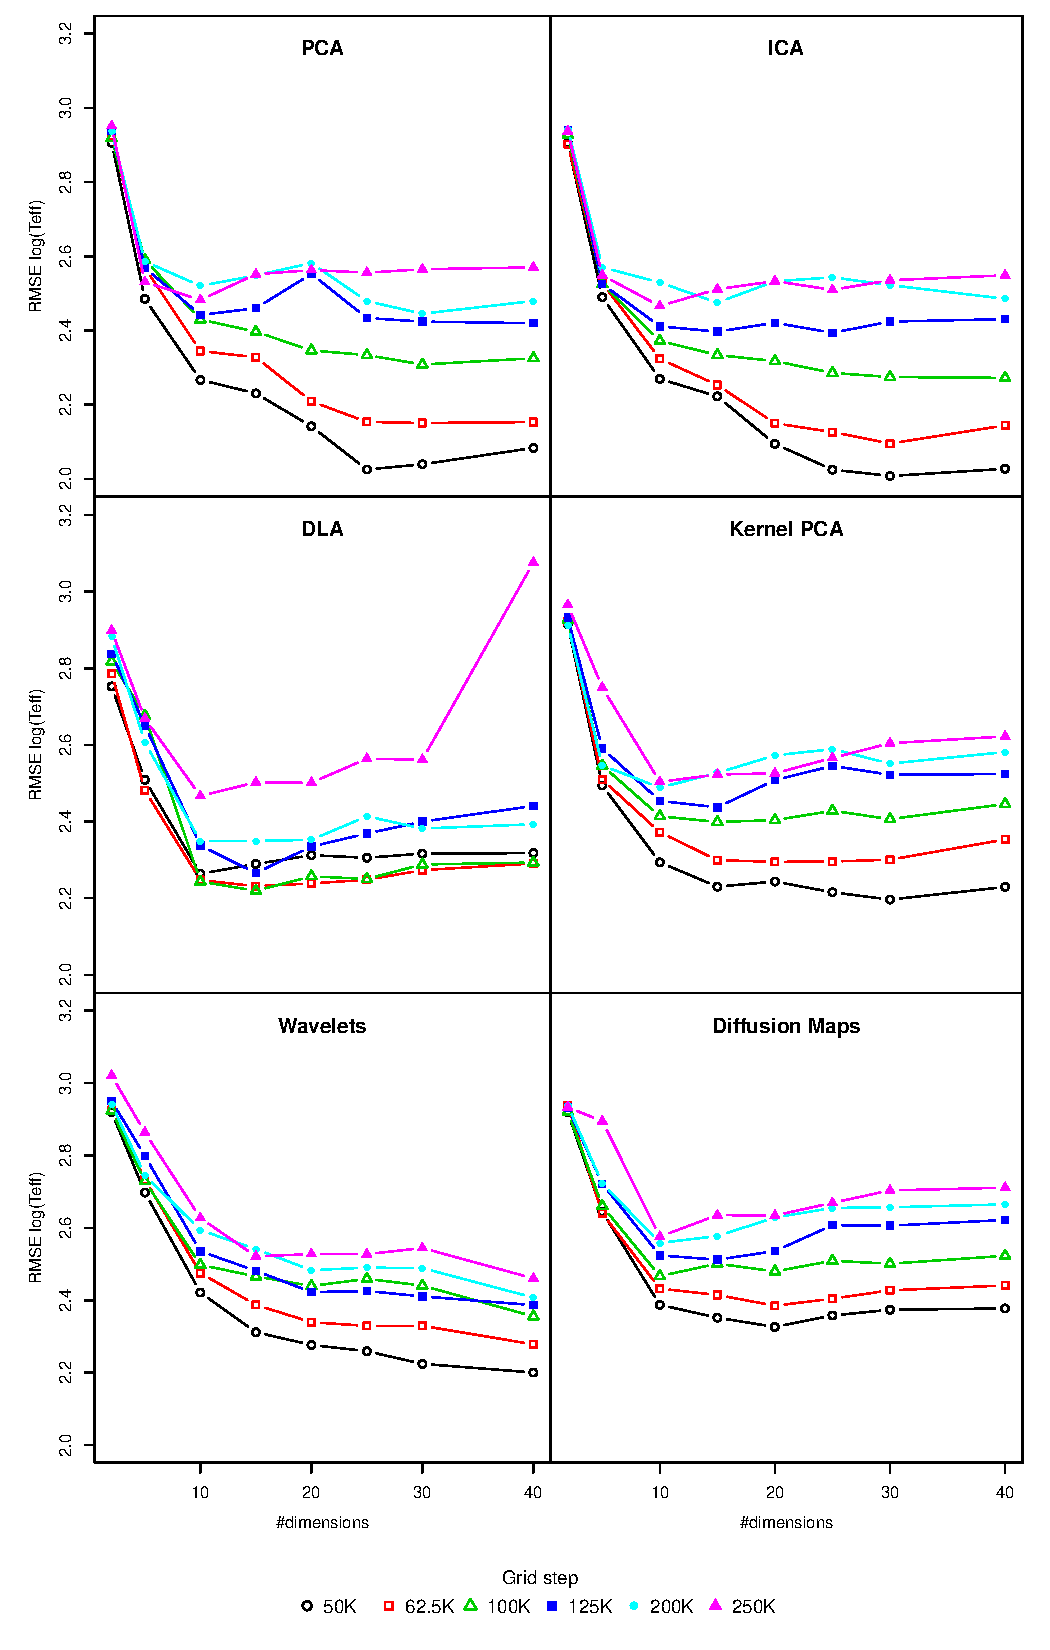
\includegraphics[height=0.95\textheight]{bestSVM_Teff_N-RMSE_HR10_snr=50_all.pdf}
\caption{Temperature estimation error against the number of dimensions
  used for data compression. Each line corresponds to a model trained
  with a specific grid step (SNR = 50)}
\label{fig:grid50}
\end{figure*}

\begin{figure*}
\centering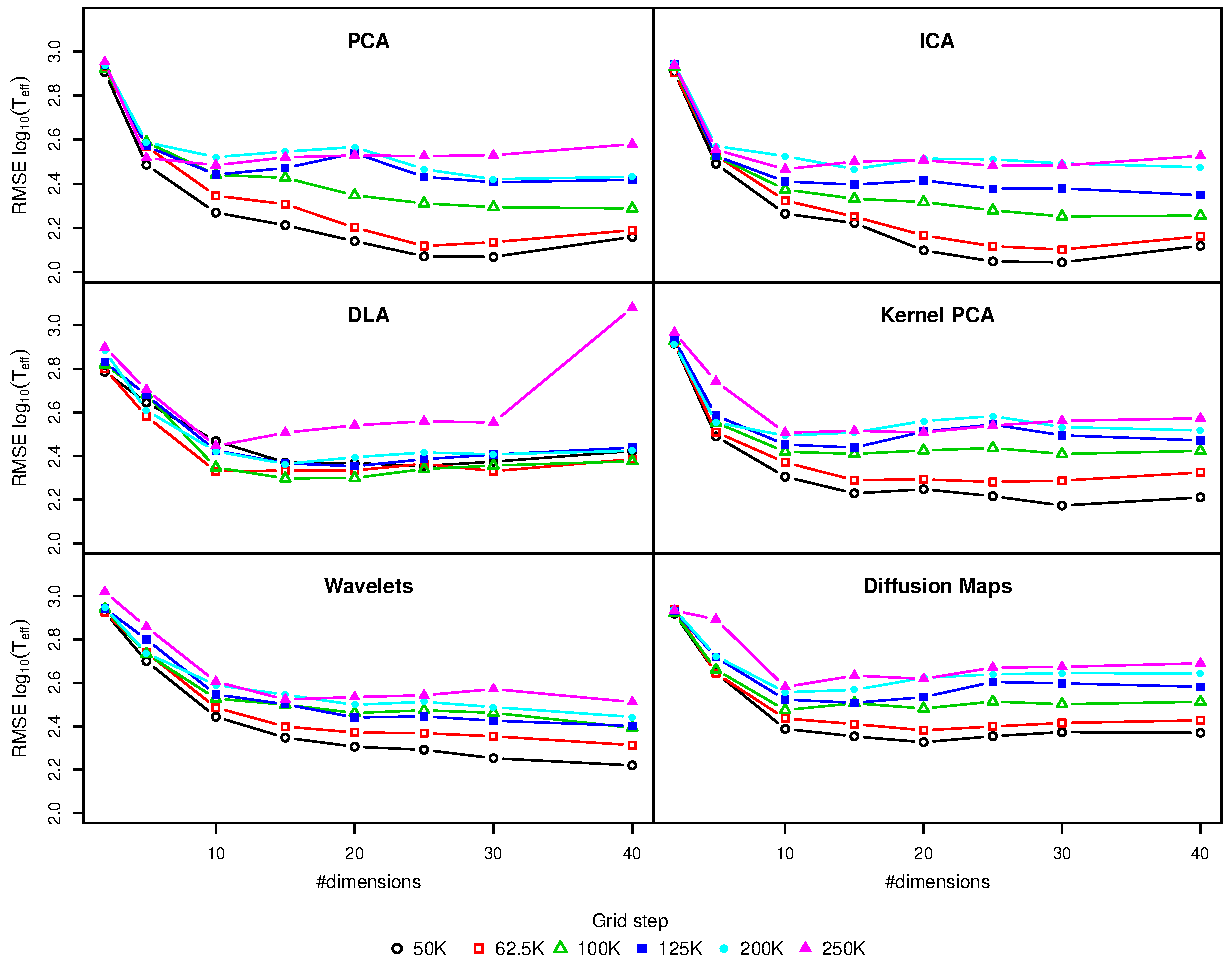
\includegraphics[height=0.95\textheight]{bestSVM_Teff_N-RMSE_HR10_snr=25_all.pdf}
\caption{Temperature estimation error against the number of dimensions
  used for data compression. Each line corresponds to a model trained
  with a specific grid step (SNR = 25)}
\label{fig:grid25}
\end{figure*}

\begin{figure*}
\centering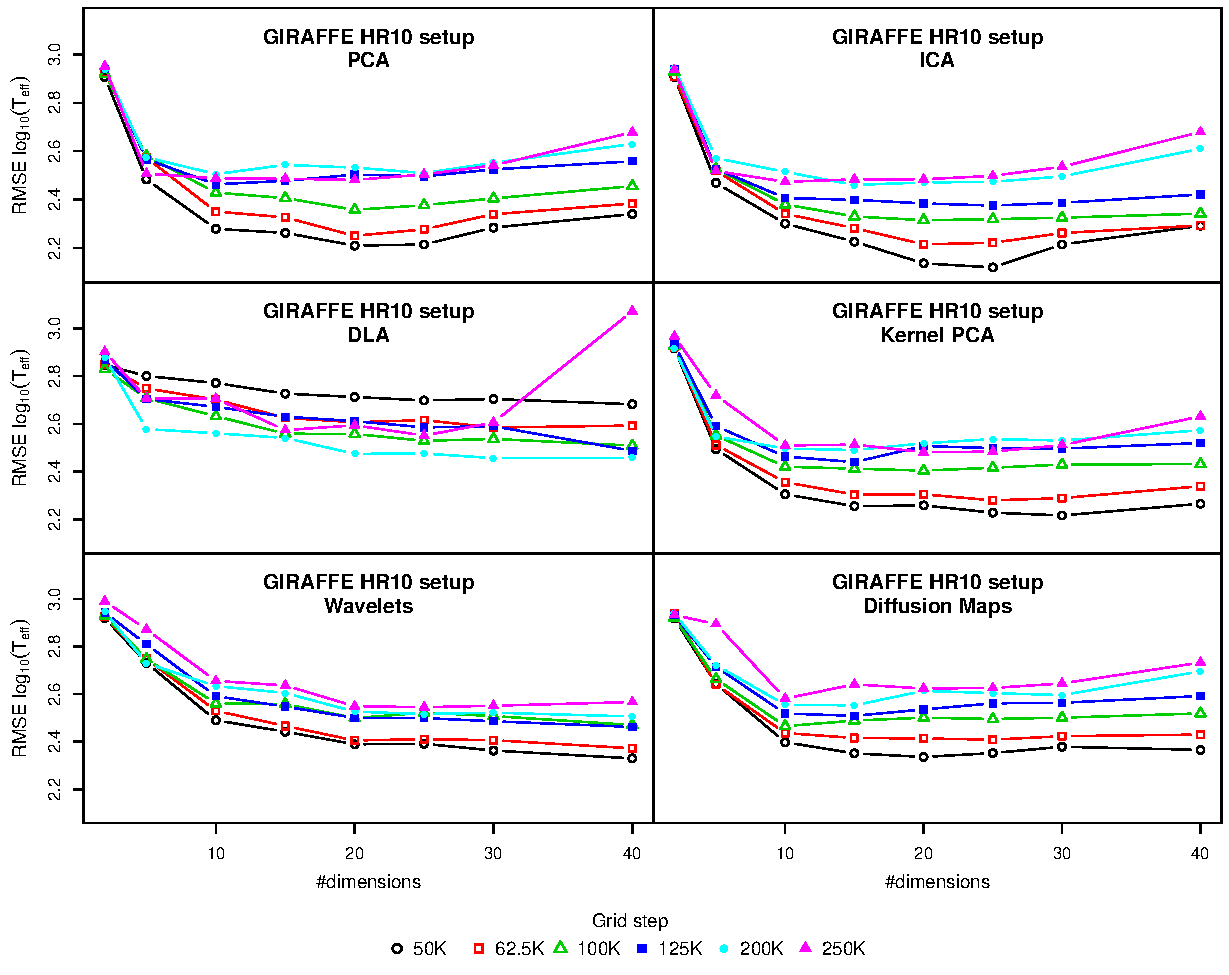
\includegraphics[height=0.95\textheight]{bestSVM_Teff_N-RMSE_HR10_snr=10_all.pdf}
\caption{Temperature estimation error against the number of dimensions
  used for data compression. Each line corresponds to a model trained
  with a specific grid step (SNR = 10)}
\label{fig:grid10}
\end{figure*}


\section{Conclusions}
\label{sec:conclusions}

{\bf Here we should discuss the validity of our conclusions. The
  validity depends on our assumptions and the experiments carried
  out. For example, they are based on SVM models with radial kernel
  functions and the implications should be stressed. Also the spectra
  were trimmed in a wavelength range: how is this range? Also compare
  our RMSE with those in the bibliography, for example, those of
  MATISSE, the Gaia-ESO results...}

\section*{Acknowledgements}
This research was supported by the Spanish Ministry of Economy and Competitiveness through grant AyA2011-24052. 



%%%%%%%%%%%%%%%%%%%%%%%%%%%%%%%%%%%%%%%%%%%%%%%%%%

%%%%%%%%%%%%%%%%%%%% REFERENCES %%%%%%%%%%%%%%%%%%

% The best way to enter references is to use BibTeX:

\bibliographystyle{mnras}
\bibliography{references} % if your bibtex file is called example.bib


% Alternatively you could enter them by hand, like this:
% This method is tedious and prone to error if you have lots of references
%\begin{thebibliography}{99}
%\bibitem[\protect\citeauthoryear{Author}{2012}]{Author2012}
%Author A.~N., 2013, Journal of Improbable Astronomy, 1, 1
%\bibitem[\protect\citeauthoryear{Others}{2013}]{Others2013}
%Others S., 2012, Journal of Interesting Stuff, 17, 198
%\end{thebibliography}

%%%%%%%%%%%%%%%%%%%%%%%%%%%%%%%%%%%%%%%%%%%%%%%%%%

%%%%%%%%%%%%%%%%% APPENDICES %%%%%%%%%%%%%%%%%%%%%

\appendix

\section{Some extra material}

If you want to present additional material which would interrupt the flow of the main paper,
it can be placed in an Appendix which appears after the list of references.

%%%%%%%%%%%%%%%%%%%%%%%%%%%%%%%%%%%%%%%%%%%%%%%%%%


% Don't change these lines
\bsp	% typesetting comment
\label{lastpage}
\end{document}

% End of mnras_template.tex